\documentclass[11pt,a4paper]{article}

\usepackage[utf8]{inputenc}
\usepackage[T1]{fontenc}
\usepackage{lmodern}
\usepackage[margin=2.3cm]{geometry}
\usepackage{amsmath,amssymb,amsthm,mathtools}
\usepackage{graphicx}
\usepackage{booktabs}
\usepackage{array}
\usepackage{microtype}
\usepackage{xcolor}
\usepackage{hyperref}

\hypersetup{
  colorlinks=true,
  linkcolor=blue!55!black,
  citecolor=teal!60!black,
  urlcolor=blue!60!black,
  pdftitle={Observer-Separated Two-Time Quantum Dynamics: Local Horizon Obstructions, Cross-Perspective Consistency, and Finite-Dimensional Evaporation Bounds},
  pdfauthor={Yohtaro Soga}
}

\newtheorem{theorem}{Theorem}
\newtheorem{proposition}[theorem]{Proposition}
\newtheorem{corollary}[theorem]{Corollary}
\newtheorem{lemma}[theorem]{Lemma}
\theoremstyle{definition}
\newtheorem{definition}{Definition}
\theoremstyle{remark}
\newtheorem{remark}{Remark}

\newcommand{\Tr}{\operatorname{Tr}}
\newcommand{\id}{\mathrm{id}}
\newcommand{\ad}{\operatorname{ad}}
\newcommand{\cH}{\mathcal{H}}
\newcommand{\cA}{\mathcal{A}}
\newcommand{\cD}{\mathcal{D}}
\newcommand{\cL}{\mathcal{L}}
\newcommand{\cE}{\mathcal{E}}
\newcommand{\cR}{\mathcal{R}}
\newcommand{\cP}{\mathcal{P}}
\newcommand{\cF}{\mathcal{F}}
\newcommand{\cU}{\mathcal{U}}
\newcommand{\cI}{\mathcal{I}}
\newcommand{\bbC}{\mathbb{C}}
\newcommand{\bbR}{\mathbb{R}}
\newcommand{\1}{\mathbf{1}}
\newcommand{\normF}[1]{\|#1\|_F}
\newcommand{\code}[1]{{\footnotesize\ttfamily #1}}

\title{\textbf{Observer-Separated Two-Time Quantum Dynamics:\\
Local Horizon Obstructions, Cross-Perspective Consistency,\\
and Finite-Dimensional Evaporation Bounds}}

\author{Yohtaro Soga\thanks{Independent researcher. Correspondence: \href{mailto:gawakkyu0603@gmail.com}{gawakkyu0603@gmail.com}. Author contributions and AI assistance are disclosed in the Author Contributions and AI Disclosure section.}}

\date{November 28, 2026}

\begin{document}
\maketitle
\vspace{-1.2em}
\begin{abstract}\footnotesize
We pose an operational tension of black hole evaporation as a structural clue toward quantum gravity: once Hawking radiation is included, an infalling observer $A$ crosses a macroscopic Schwarzschild horizon in finite proper time encountering locally smooth vacuum, whereas a distant asymptotic observer $B$'s directly accessible records contain only exponentially redshifted signals and outgoing radiation dispersing $A$'s degrees of freedom. Guided by this divergence of accessible futures, we formulate \emph{Observer-Separated Two-Time Quantum Dynamics} (OSTQD) on finite-dimensional matrix algebras, separating reversible unitary clock evolution ($t \in \bbR$) from purely dissipative, non-selective auxiliary-time evolution ($s \in [0,\infty)$, analogous in parameter structure to Parisi--Wu stochastic time) indexed by observer perspectives $O$ and accessible subalgebras $\cA_O$.

We prove five conditional finite-dimensional theorems whose algebraic core (50~audited public declarations) is machine-checked in Lean~4.36.0 with Mathlib4 (zero \texttt{sorry}, zero tactic-linter warnings, standard axioms only) and audited numerically in Python (451~recorded numeric fields, strictly separating algebraic proofs from analytic steps and physical hypotheses):
(1)~Specifying global-state algebra restriction vs.\ autonomous subalgebra closure ($[H_O,\cA_O]\subseteq\cA_O$, illustrated by a $D_2\otimes M_2$ non-closure counterexample), we show from $\Gamma_{\cL}(H,H) = \sum_k [L_k,H]^\dagger [L_k,H]$ that zero first- and second-moment energy drift holds iff $[L_k,H]=0$ for all $k$, which is sufficient (not necessary) for $(t,s)$ commutation $[\cL,\ad_H]=0$, while $\frac{1}{d}\Tr(\Gamma_{\cL}(H,H))$ equals the exact eigenbasis-averaged initial variance rate $\frac{1}{d}\sum_j \partial_s \mathrm{Var}_{|E_j\rangle}(H)|_{s=0}$ rather than $\partial_s\mathrm{Var}_{\rho_{\mathrm{mm}}}(H)$.
(2)~Whenever $\cA_O \cap \{H_A,H_B\}' = \bbC\1$, no nontrivial $H_A$- and $H_B$-BPS-immune generator exists in $\cA_O$, and $H_B$-BPS-immune flows satisfy an eigenbasis-averaged variance bound governed by $\gamma_{\mathrm{loc}}(H_A,H_B;\cA_O)$. While $[H_A,H_B]=0$ globally on the 4D two-sided fermionic Hawking pair, restricting to $\cA_B = M_2(\bbC)_R\otimes\1_L$ gives $\gamma_{\mathrm{loc}} = 8\omega^2 n_{\mathrm{FD}}(1-n_{\mathrm{FD}})$ ($T_H>0$) and excites the two-sided observable $H_A$ on $|0_A\rangle$ at rate $2\Gamma\omega\,n_\sigma(1+\sigma n_\sigma)$ ($\sigma=\pm 1$), saturating at $\langle H_A\rangle_{\rho_B(\infty)}/(2\omega) = \normF{\rho_0 - \cP_B(\rho_0)}^2 = S_L(\rho_R^{\mathrm{Hawking}})$ for fermions while leaving both one-sided reduced states $\Tr_L\rho_B(s)$ and $\Tr_R\rho_B(s)$ invariant; a 4D counterexample shows $\gamma_{\mathrm{loc}}>0$ alone does not force ground-state heating without the entangled vacuum structure.
(3)~For $d_C\ge 2$, any global joint CPTP extension on $(\bbC^{d_C})^{\otimes 3}$ obeys the Kay--Kaszlikowski--Ramanathan / Nechita--Pellegrini--Rochette curved upper/lower boundaries---with the entire shaded band constructively attained by valid CPTP Choi states---and the sharp linear outer envelope $F_A+F_B \le 1+1/d_C$, whereas separate-condition reversible encodings $(\cE_A,\cE_B)$ attain $F_e=1$ each with marginal agreement on a shared factor $\cA_{\mathrm{sh}}$, supplemented by a causal projective shared-record readout ($P(x\neq y)=0$, matching the $s\to\infty$ record limit) contrasted with finite-$s$ weak measurement.
(4)~Hermitian-jump flows decrease purity monotonically, satisfy $S_L(\cP(\rho)) = S_L(\rho)+\|\rho-\cP(\rho)\|_F^2$ with $e^{s\cL}\to\cP$ for sector-separating commuting jumps, and reconcile non-stationary intra-window $t$-evolution with exact $s$-invariance inside a finite-width energy window $\Pi_{\mathrm{win}}$.
(5)~Specializing Farber and Gour's unassisted single-shot quantum compression theorem to maximally mixed inputs, we give an elementary Lean-verified Kraus proof (covering both $d_f\le d_C$ and $d_f>d_C$) of $F_e(\cR\circ\cE) \le \min(1, d_f^2/d_C^2)$, audit its no-classical-side-channel resource requirement via a 1-bit flag counterexample ($F_e=1/2>1/4$), and present a two-window $t$-encoding/$s$-invariance evaporation example alongside a fixed-cutoff $SU(2)$ Yang--Mills Galerkin benchmark.
\end{abstract}

\newpage
\tableofcontents
\vspace{1em}

%==============================================================================
\section{Introduction}\label{sec:intro}
%==============================================================================

\subsection{Conceptual Origin: The Hawking-Evaporation Observer-Discrepancy Paradox}\label{sec:origin}

The conceptual starting point of this work is a foundational physical question raised by black hole evaporation: \emph{when Hawking radiation is taken into account, the future of a physical object falling into a black hole does not match across different observers' viewpoints; how can this observer-dependent divergence itself be incorporated as a structural clue toward a theory of quantum gravity?}

Concretely, consider an infalling observer $A$ carrying an unknown quantum system $C$ of Hilbert-space dimension $d_C \ge 2$ freely falling into a macroscopic Schwarzschild black hole of mass $M$, while a distant observer $B$ remains in the asymptotically flat exterior. In semiclassical general relativity, $A$ crosses the event horizon in finite proper time $\tau_A \sim r_s / c$, encountering locally inertial vacuum and curvature $\mathcal{O}(r_s^{-2})$, and continues smoothly into the interior. By contrast, signals sent from $A$ to $B$ suffer exponential gravitational redshift: while coordinate-time divergence $dt/d\tau \to \infty$ in static Schwarzschild coordinates is itself a coordinate artifact (regular advanced coordinates $v = t + r_*$ remain smooth across horizon crossing, and semiclassical causal diagrams of finite-time evaporation still contain an interior spacetime region \cite{UnruhWald2017}), two logically distinct ingredients must be kept separate once Hawking evaporation \cite{Hawking1975,Page1976,Page1993} is included. First, as a causal fact, $B$'s \emph{directly accessible asymptotic records} receive no direct signal from inside the horizon; second, as an additional dynamical assumption of exterior unitarity, outgoing radiation eventually disperses the mass $M$ in finite asymptotic time $t_{\mathrm{evap}} \sim M^3$ (in Planck units) and enables decoding of $C$'s quantum information under conditions that depend on injection time, initial black-hole entanglement, and access to the emitted radiation (e.g., rapid release after the Page time for an old maximally entangled black hole \cite{HaydenPreskill2007,Penington2020,AlmheiriIslands2020}). Likewise, whenever fixed Killing-generator single-mode calculations are applied to an evaporating spacetime, they serve strictly as stationary or adiabatic local approximations.

In classical general relativity, differing coordinate slicings pose no logical contradiction because both worldlines embed smoothly into a single classical Lorentzian manifold. Once quantum mechanics and Hawking evaporation are combined, however, reconciling $A$'s locally smooth interior records with exterior unitarity and semiclassical effective field theory triggers sharp quantum-information tensions: the cloning/complementarity puzzle \cite{Susskind1993,Nomura2013,Nomura2013PRD} and the Almheiri--Marolf--Polchinski--Sully (AMPS) firewall paradox \cite{AMPS2013}.

Treating this evaporation-induced mismatch between accessible interior and exterior futures not merely as an obstacle to be eliminated, but as a structural principle for dynamics, directly motivates the guiding hypothesis of OSTQD: \emph{quantum dynamics may require explicitly separating reversible unitary evolution (along physical/clock time $t \in \bbR$) from irreversible, observer-relative non-selective dissipative evolution (along a directed auxiliary parameter $s \in [0,\infty)$, analogous in mathematical structure to Parisi--Wu fictitious stochastic time \cite{ParisiWu1981}), so that each observer's reversible dynamics and irreversible dissipation structure are indexed by that observer's accessible algebra $\cA_O$ and clock generator $H_O$.} Our strategy is to distill this conceptual proposal into a sequence of precise, finite-dimensional mathematical constructions and conditional theorems where every assumption, counterexample, and limitation can be tested rigorously.

\subsection{Contemporary Theoretical Landscape (2022--2026)}\label{sec:landscape}

Four major recent developments frame the mathematical context in which this hypothesis must be evaluated:
\begin{enumerate}
  \item \textbf{Observer-dependent gravitational algebras and quantum reference frames:} Dressing observables to a dynamical observer's clock via crossed products promotes semiclassical Type~$\mathrm{III}_1$ subalgebras to Type~$\mathrm{II}_1$ or Type~$\mathrm{II}_\infty$ factors with well-defined traces and observer-dependent generalized entropies (e.g., the de~Sitter static-patch Type~$\mathrm{II}_1$ algebra gravitationally dressed to an observer's worldline \cite{CLPW2023}, alongside general-subregion and crossed-product analyses \cite{CPW2023,JensenSorceSperanza2023,KudlerFlam2023,DeVuyst2024,DeVuyst2025}). In a related line of work, comparisons of R\'enyi entropies and diagonal invariants across quantum reference frames clarify how reduced entropies transform between perspectives \cite{delaHamette2026}.
  \item \textbf{Firewall paradox as Wigner's friend paradox:} Extending no-go theorems on observer-independent facts \cite{FrauchigerRenner2018,Bong2020} and cross-perspective links (CPL) in relational quantum mechanics \cite{Rovelli1996,AdlamRovelli2022}, recent analyses \cite{HausmannRenner2025,Walleghem2025,Adlam2026} argue that the AMPS firewall paradox relies on an implicit perspective-combining rule already challenged in extended Wigner's friend scenarios.
  \item \textbf{Non-isometric holographic encodings, single-shot compression, and matrix black holes:} Building on holographic quantum error correction \cite{AlmheiriDongHarlow2015}, late-time interior-to-exterior maps with more effective bulk states than fundamental black hole microstates are modeled as non-isometric linear codes \cite{Akers2022}; in finite-dimensional quantum information, exact unassisted vs.\ classically assisted single-shot quantum compression bounds were recently characterized via Ky Fan norms \cite{FarberGour2026}, alongside microscopic matrix-model studies of black 0-branes \cite{BFSS1997,IKKT1997,Choudhury2024}.
  \item \textbf{Conservation laws, detector-field coupling, decoherence--diffusion trade-offs, and precision bounds:} Banks, Susskind, and Peskin (BPS) \cite{BPS1984} demonstrated that universal pure-to-mixed master equations generically clash with energy conservation or locality; subsequent work established the continuous Wigner--Araki--Yanase (WAY) theorem \cite{KuramochiTajima2023}, decoherence--diffusion trade-offs in hybrid classical--quantum gravity \cite{Oppenheim2023PRX,Oppenheim2023NC,TilloyDiosi2016,Stamp2015}, explicit accelerated-detector vs.\ inertial particle-creation analyses \cite{UnruhWald1984}, Killing-horizon-induced decoherence \cite{DSW2023}, stringent laboratory bounds on universal collapse \cite{Donadi2021,Pedalino2025}, and precision tests of the weak equivalence principle on composition-dependent free-fall accelerations \cite{MICROSCOPE2022} (which constrain specific collapse models only once a concrete coupling prescription is supplied; cf.\ Remark~\ref{rem:horizon-scope}).
\end{enumerate}

\subsection{Main Contributions, Inherited Tools, and Open Problems}\label{sec:novelty}

To delineate the scientific contributions of this work clearly and avoid conflating established operator-algebraic or quantum-information theorems with new constructions or unproven quantum-gravity claims, we organize our results into four tiers:

\begin{enumerate}
  \item \textbf{Conceptual Proposal, Concrete Constructions, and Formalized Synthesis} (distinguishing our conceptual framing, specific finite-dimensional constructions, and observer-indexed synthesis from broader priority claims over general quantum-Markov, DFS, cloning, or single-shot compression theory):
  \begin{itemize}
    \item \emph{Paradox-motivated conceptual formulation and $(t,s)$ synthesis:} Posing the operational divergence between an infalling observer's locally smooth interior evolution and an asymptotic observer's directly accessible evaporation records as a structural clue toward quantum gravity, and formulating an observer-indexed two-time framework $(\cA_O, H_O, \cL_O)$ with explicit separation of global-state algebra restriction vs.\ autonomous subalgebra closure ($[H_O,\cA_O]\subseteq\cA_O$, audited via a $D_2\otimes M_2$ non-closure counterexample).
    \item \emph{Exact eigenbasis-averaged variance-injection identity (Theorem~\ref{thm:bps}(e)--(f)):} Deriving the variance-derivative decomposition $\partial_s\mathrm{Var}_\rho(H) = \allowbreak \langle\Gamma_{\cL}(H,H)\rangle_\rho + \langle\{H,D\}\rangle_\rho - 2\langle H\rangle_\rho\langle D\rangle_\rho$, showing via explicit counterexample why $\langle\Gamma_{\cL}(H,H)\rangle_{\rho_{\mathrm{mm}}}$ does not in general equal $\partial_s\mathrm{Var}_{\rho_{\mathrm{mm}}}(H)$, and proving that $\frac{1}{d}\Tr(\Gamma_{\cL}(H,H))$ instead equals the eigenbasis-averaged initial variance rate $\frac{1}{d}\sum_j \partial_s\mathrm{Var}_{|E_j\rangle}(H)|_{s=0}$.
    \item \emph{Subalgebra-restricted horizon incompatibility and exact 4D fermionic Hawking-pair identities (Theorem~\ref{thm:horizon}(a)--(b),(e)--(f)):} Proving explicitly that $[H_A,H_B]=0$ on the full two-sided algebra $M_4(\bbC)$ (so global irreducibility fails), then proving that causal restriction to the exterior local algebra $\cA_B = M_2(\bbC)_R\otimes\1_L$ restores irreducibility ($\cA_B\cap\{H_A,H_B\}'=\bbC\1$ for $T_H>0$), yields the closed-form local incompatibility $\gamma_{\mathrm{loc}}(H_A,H_B;\cA_B) = \allowbreak 8\omega^2 n_{\mathrm{FD}}(1-n_{\mathrm{FD}})$, yields the unified single-mode vacuum excitation rate $\partial_s\langle H_A\rangle|_{s=0} = \allowbreak 2\Gamma\omega\,n_\sigma(1+\sigma n_\sigma) = \allowbreak 2\Gamma\omega\,\mathrm{Var}_{|0_A\rangle}(N_R)$ ($\sigma=\pm 1$), and yields the $s\to\infty$ fermionic saturation identity $\langle H_A\rangle_{\rho_B(\infty)}/(2\omega) = \allowbreak \normF{\rho_0 - \cP_B(\rho_0)}^2 = \allowbreak S_L(\rho_R^{\mathrm{Hawking}})$ ($\rho_0 := |0_A\rangle\langle 0_A|$) alongside explicit proofs of one-sided reduced-state invariance and a 4D counterexample separating $\gamma_{\mathrm{loc}}>0$ from ground-state excitation.
    \item \emph{Complete achievable joint-channel band, CPTP Choi constructions, and projective vs.\ weak shared-record readout (Theorem~\ref{thm:cpl}):} Establishing valid CPTP Choi saturation across the entire shaded achievable region---the curved upper boundary $\sigma^+(x)$, curved lower boundary $\sigma^-(x)$, flat zero lower boundary via a shift measure-and-prepare channel, and all interior points via convex mixtures (distinguishing Kay et al.'s local-unitary-maximized singlet fraction \cite{Kay2009} from the full covariant cloning region of Nechita, Pellegrini, and Rochette \cite{Nechita2021})---separating expectation-value marginal consistency from single-trial record agreement, and constructing an explicit causal projective shared-record readout ($P(x\neq y)=0$, matching the $s\to\infty$ record-dephasing limit) contrasted with finite-$s$ weak measurement.
    \item \emph{Coarse-grained finite-width energy-window compatibility with $t$-evolution (Theorem~\ref{thm:double}(e)--(f) and Section~\ref{sec:matrix}):} Proving exact spectral block decay linking $\lim_{s\to\infty} e^{s\cL} = \cP$ for sector-separating commuting Hermitian jumps, demonstrating how a finite-width energy window $\Pi_{\mathrm{win}}=\1_{[E-\Delta,E+\Delta]}(H_B)$ reconciles non-stationary intra-window $t$-evolution with exact $s$-invariance (illustrated alongside an inter-window $s$-decay contrast and a two-logical-qubit bottleneck check).
    \item \emph{Auditable formal and numerical verification:} Machine-checking the finite-dimensional algebraic core (50~audited public declarations) in Lean~4.36.0 + Mathlib4 (zero tactic-linter warnings; clean kernel log in \code{lean4/\allowbreak VERIFICATION\_\allowbreak LOG.txt}) paired with a deterministic self-checking Python suite (451~numeric fields, pinned \code{scripts/requirements.txt}).
  \end{itemize}
  \item \textbf{Inherited Mathematical Tools and Specializations of Prior Art (Explicitly Attributed):}
  The GKSL master equation and BPS conservation criterion \cite{Lindblad1976,GKS1976,BPS1984} (Theorem~\ref{thm:bps}(a)--(d)); the exact curved singlet-monogamy / optimal cloning boundary of Kay, Kaszlikowski, and Ramanathan \cite{Kay2009} and the full universal asymmetric cloning region of Nechita, Pellegrini, and Rochette \cite{Nechita2021} (Theorem~\ref{thm:cpl}(a)--(c)); the relative-entropy coherence decomposition of Baumgratz, Cramer, and Plenio \cite{Baumgratz2014} and decoherence-free subspaces (DFS) of Lidar, Chuang, and Whaley \cite{Lidar1998} (Theorem~\ref{thm:double}(b),(d)); Schumacher entanglement fidelity \cite{Schumacher1996}, the Petz transpose map \cite{Petz1986}, Hawking's classical area theorem \cite{Hawking1971}, and \textbf{Farber and Gour's unassisted single-shot quantum compression theorem \cite{FarberGour2026}} (§IV, Theorem~5: optimal unassisted source fidelity equals the Ky Fan norm $\|\rho\|_{(d_f)}$, whose square specializes at maximally mixed input $\rho=\1_{d_C}/d_C$ to Theorem~\ref{thm:bottleneck}'s $F_e\le\min(1,d_f^2/d_C^2)$, where our contribution is the elementary Kraus proof, Lean formalization across both $d_f\le d_C$ and $d_f>d_C$, explicit classical-flag resource audit, and conditional remnant application).
  \item \textbf{Explicit Physical Hypotheses (Not Derived from First Principles Here):}
  (i)~Causal restriction of exterior jump operators to $\cA_B = M_2(\bbC)_R\otimes\1_L$; (ii)~the physical mapping between auxiliary parameter $s$, proper time $\tau$, normalized wavepacket/detector coupling, and rate $\Gamma_O$ (yielding effective rate $\Gamma_{\mathrm{eff}}(\tau)=\Gamma_O\,ds/d\tau$, without yet distinguishing the single-mode channel from standard unitary environmental phase noise); (iii)~the operational rule governing when a global joint CPTP extension is waived in the absence of a common causal future; and (iv)~identifying finite-dimensional $\ln d_f$ with Bekenstein--Hawking entropy $S_{\mathrm{BH}}$ under strict absence of radiation or classical side-channel access.
  \item \textbf{Open Nonperturbative Problems (Explicitly Unsolved Here):}
  Extension to infinite-dimensional Type~$\mathrm{II}_1/\mathrm{II}_\infty$ crossed-product von Neumann algebras (requiring explicit trace, generator domain, and continuity data); continuum QFT stress-energy, Hadamard regularity, and wavepacket detector response; general observer-separated selective single-shot quantum instruments $\{\cI_{O,x}\}$ and causal record-merging rules beyond our shared-record factor example; microscopic derivation of $\Gamma_O$ from large-$N$ BFSS/IKKT matrix dynamics; and emergence of a smooth 4D Lorentzian manifold.
\end{enumerate}

Table~\ref{tab:literature} summarizes this positioning relative to nearest prior frameworks.

\begin{table}[!tb]
\centering\footnotesize
\caption{Positioning of OSTQD relative to nearest prior frameworks, explicitly distinguishing inherited tools and specializations of prior art, specific constructions and formalizations presented here, and remaining physical assumptions.}
\label{tab:literature}
\begin{tabular}{@{}>{\raggedright\arraybackslash}p{0.19\linewidth}>{\raggedright\arraybackslash}p{0.26\linewidth}>{\raggedright\arraybackslash}p{0.29\linewidth}>{\raggedright\arraybackslash}p{0.18\linewidth}@{}}
\toprule
Prior framework & Inherited / established contribution & Specific constructions / contributions presented here & Explicit additional assumption / limit \\
\midrule
GKSL \& BPS / WAY \cite{Lindblad1976,GKS1976,BPS1984,KuramochiTajima2023} & GKSL structure and conservation obstructions for universal mixed evolution. & Algebra-closure vs.\ restriction audit ($D_2\otimes M_2$ counterexample), eigenbasis-averaged variance rate (Thm.~\ref{thm:bps}(e)--(f)), and $\gamma_{\mathrm{loc}}$ (Thm.~\ref{thm:horizon}(a)--(b)). & Finite dimensions; jump locality $\cA_B$ imposed as physical axiom. \\
Observer algebras, Unruh/Hawking \& decoherence \cite{Hawking1975,Unruh1976,UnruhWald1984,CLPW2023,DeVuyst2024,DeVuyst2025,delaHamette2026,DSW2023} & Observer-dressed Type~II algebras, QRF R\'enyi comparisons, detector-field coupling, horizon decoherence. & Explicit proof that $[H_A,H_B]=0$ on $M_4(\bbC)$ while $\cA_B$-restriction gives $\gamma_{\mathrm{loc}}=8\omega^2 n_{\mathrm{FD}}(1-n_{\mathrm{FD}})$, fermionic saturation, reduced-state invariance, and fixed-ground-state counterexample (Thm.~\ref{thm:horizon}). & Single-mode channel (equivalent to phase noise); wavepackets, $\langle T_{\mu\nu}\rangle$, \& Type~II open. \\
Cloning, Wigner's friend \& CPL \cite{Kay2009,Nechita2021,FrauchigerRenner2018,Bong2020,AdlamRovelli2022,HausmannRenner2025,Walleghem2025,Adlam2026} & Curved singlet monogamy \cite{Kay2009} \& full universal cloning region \cite{Nechita2021}; AMPS linked to Wigner's friend; CPL. & Short projection proof \& Lean-checked CPTP Choi attainment of the full shaded band (upper, lower, interior), marginal CPL witness, and projective readout vs.\ finite-$s$ weak measurement (Thm.~\ref{thm:cpl}). & Shared-factor model; general black-hole record-merging rules remain open. \\
Coherence, DFS, single-shot compression, non-isometric codes \& BH area \cite{Baumgratz2014,Lidar1998,Schumacher1996,FarberGour2026,Akers2022,Hawking1971} & Relative-entropy coherence, DFS, unassisted single-shot compression $\|\rho\|_{(m)}^2$ \cite{FarberGour2026}, non-isometric codes, area theorem. & Spectral block decay $e^{s\cL}\to\cP$, finite-width window compatibility + inter-window $s$-contrast, and Lean-checked Kraus proof ($d_f\le d_C$ \& $d_f>d_C$) + 1-bit classical-flag audit of the $\rho=\1/d_C$ case of \cite{FarberGour2026} (Thm.~\ref{thm:bottleneck}). & No classical side channel or radiation access; $\ln d_f\leftrightarrow S_{\mathrm{BH}}$ is an assumption. \\
\bottomrule
\end{tabular}
\end{table}

%==============================================================================
\section{Observer-Separated Two-Time Quantum Dynamics (OSTQD)}\label{sec:framework}
%==============================================================================

\paragraph{Conventions and units.}
Throughout this paper we work in natural units $\hbar = k_B = 1$ unless explicitly noted. Logarithms in dimensional formulas ($\ln d_C$, $\ln d_f$) and analytic von Neumann entropies $S(\rho) := -\Tr(\rho\ln\rho)$ are natural logarithms (nats); in Figure~\ref{fig:matrix}(a) we explicitly divide by $\ln 2$ to display entanglement entropy in bits. The mode frequency $\omega$ and Hawking temperature $T_H$ carry energy units; the auxiliary dissipation parameter $s \ge 0$ and rate constant $\Gamma$ are chosen such that $\Gamma s$ is dimensionless (for instance, if $s$ has dimensions of time, $\Gamma$ has dimensions of inverse time). Whenever an asymptotic $s \to \infty$ limit is taken, we require strictly positive coupling $\Gamma > 0$. Whenever traceless incompatibility constants $\gamma$ or $\gamma_{\mathrm{loc}}$ are defined via an infimum over nonzero traceless operators, we require Hilbert-space dimension $d \ge 2$ (for $d = 1$ the traceless subspace is trivial).

We formulate OSTQD in finite-dimensional Hilbert spaces $\cH \cong \bbC^d$ (with a truncated bosonic Fock-space extension in Section~\ref{sec:horizon}) so that every operator identity is unconditionally rigorous and free of unbounded-operator domain ambiguities.

\begin{definition}[Observer Perspective, Algebra-Evolution Relation, Integrable Two-Time Dynamics, and State Levels]\label{def:ostqd}
Let $\cH \cong \bbC^d$ ($d \ge 2$) be a finite-dimensional Hilbert space equipped with the Hilbert--Schmidt inner product $\langle X, Y\rangle_{\mathrm{HS}} := \Tr(X^\dagger Y)$ and Frobenius norm $\normF{X}^2 := \Tr(X^\dagger X) = \sum_{i,j}|X_{ij}|^2$. An \emph{observer perspective} $O \in \mathcal{O}$ is specified by:
\begin{enumerate}
  \item an accessible observable $C^*$-subalgebra $\cA_O \subseteq M_d(\bbC)$ containing $\1$;
  \item a Hermitian clock/energy Hamiltonian $H_O = H_O^\dagger \in M_d(\bbC)$ generating reversible unitary evolution $\cU_O(t)(\rho) := e^{-iH_O t}\rho\, e^{iH_O t}$ on $M_d(\bbC)$ in physical/clock time $t \in \bbR$ (with Heisenberg dual $\cU_O^\dagger(t)(X) = e^{iH_O t} X e^{-iH_O t}$);
  \item a finite family of jump operators $\{L_{O,k}\}_{k=1}^m \subset \cA_O$ defining the \emph{purely dissipative} (no auxiliary-time Hamiltonian term) Gorini--Kossakowski--Sudarshan--Lindblad (GKSL) \cite{Lindblad1976,GKS1976} non-selective dissipative generator
  \begin{equation}\label{eq:gksl}
    \cL_O(\rho) := \sum_{k=1}^m \left(L_{O,k}\rho L_{O,k}^\dagger - \tfrac{1}{2}\bigl\{L_{O,k}^\dagger L_{O,k},\,\rho\bigr\}\right),
  \end{equation}
  and its Heisenberg dual $\cL_O^\dagger(X) := \sum_{k=1}^m \bigl(L_{O,k}^\dagger X L_{O,k} - \frac{1}{2}\{L_{O,k}^\dagger L_{O,k}, X\}\bigr)$, generating the completely positive, trace-preserving (CPTP) semigroup $\Phi_O(s) = e^{s\cL_O}$ along a directed \emph{auxiliary parameter} $s \in [0,\infty)$. Since $L_{O,k}\in\cA_O$, the auxiliary flow always preserves $\cA_O$: $\cL_O^\dagger(\cA_O)\subseteq\cA_O$ and $\Phi_O^\dagger(s)(\cA_O)\subseteq\cA_O$.
\end{enumerate}
\emph{Algebra--evolution specification:} Because $\cU_O(t)$ acts on the full matrix algebra $M_d(\bbC)$, we explicitly distinguish two regimes:
(a)~\emph{Global-state restriction (default for general causal regions):} a designated total state $\rho_{\mathrm{tot},O}(0,0)\in\cD(\cH)$ is evolved on $M_d(\bbC)$, and observer $O$'s operational predictions at $(t,s)$ are defined by restricting the evolved global state to $O$'s accessible algebra $\cA_O$ (or a time/region-indexed algebra $\cA_O(t)$): $\omega_{O,t,s}(X) := \Tr(X\,\rho_{\mathrm{tot},O}(t,s))$ for $X\in\cA_O$.
(b)~\emph{Autonomous closed evolution on a fixed algebra $\cA_O$:} whenever initial expectations on $\cA_O$ alone are required to determine all future $\cA_O$-expectations without specifying the global extension outside $\cA_O$, we additionally impose $\cU_O^\dagger(t)(\cA_O)\subseteq\cA_O$ for all $t\in\bbR$ (equivalently $[H_O,\cA_O]\subseteq\cA_O$; e.g., $H_O\in\cA_O$ or $H_O=H_R+H_L$ on $\cA_B = M_{d_R}\otimes\1_L$).

Whenever the \emph{integrability (commutation) condition}
\begin{equation}\label{eq:integrability}
  \bigl[\cL_O,\,\ad_{H_O}\bigr](\rho) := \cL_O\bigl([H_O,\rho]\bigr) - \bigl[H_O,\cL_O(\rho)\bigr] = 0 \qquad \forall \rho \in M_d(\bbC)
\end{equation}
holds, the two-parameter state
\[
  \rho_{\mathrm{tot},O}(t,s) := \bigl(\cU_O(t)\circ\Phi_O(s)\bigr)\bigl(\rho_{\mathrm{tot},O}(0,0)\bigr) = \bigl(\Phi_O(s)\circ\cU_O(t)\bigr)\bigl(\rho_{\mathrm{tot},O}(0,0)\bigr)
\]
is the unique path-independent solution of the simultaneous partial differential equations
\begin{equation}\label{eq:two-time}
  \partial_t \rho_{\mathrm{tot},O}(t,s) = -i[H_O, \rho_{\mathrm{tot},O}(t,s)], \qquad
  \partial_s \rho_{\mathrm{tot},O}(t,s) = \cL_O\bigl(\rho_{\mathrm{tot},O}(t,s)\bigr).
\end{equation}
In OSTQD, we impose $H_O$-BPS immunity ($\cL_O^\dagger(H_O) = \cL_O^\dagger(H_O^2) = 0$, equivalently $[L_{O,k}, H_O]=0$ by Theorem~\ref{thm:bps}(c)) on each observer's \emph{own} perspective as a physical energy-conservation requirement---so that observer $O$'s auxiliary dissipative evolution neither heats nor cools $O$'s own clock energy distribution. This is strictly stronger than \eqref{eq:integrability} (it is sufficient, not necessary, for two-time commutation; cf.\ Remark~\ref{rem:def-precisions}) and enforces \eqref{eq:integrability} automatically by Theorem~\ref{thm:bps}(d). Because Definition~\ref{def:ostqd} permits non-Hermitian jump operators $L_{O,k}$, even under $[L_{O,k}, H_O]=0$ population transfer inside a degenerate energy eigenspace can increase purity (e.g., $H=\mathrm{diag}(0,0,1)$, $L=|0\rangle\langle 1|$, $\rho=\mathrm{diag}(3/4,1/4,0)$ satisfies $[L,H]=0$ yet $2\Tr[\rho\cL(\rho)] = +1/4 > 0$, formalized as \code{nonhermitian\_\allowbreak bps\_\allowbreak degenerate\_\allowbreak purity\_\allowbreak increase}); while general Hermitian jump flows guarantee purity non-increase (Theorem~\ref{thm:double}(a)), we reserve ``pure dephasing'' (preserving populations in a fixed eigenbasis) specifically for simultaneously diagonalizable spectral jumps (Theorem~\ref{thm:double}(e), such as $L=\sqrt{\Gamma}N_R$ in Section~\ref{sec:horizon}; by contrast, non-commuting Hermitian jumps such as $K_1=\sigma_x, K_2=\sigma_z$ in Remark~\ref{rem:coherence-window}(1) depolarize all states to $\1_2/2$). More generally, if $H_O(t)$ is piecewise time-dependent and satisfies $[\cL_O, \ad_{H_O(t)}] = 0$ on every time interval while $\cL_O$ is $t$-independent, then the time-ordered unitary propagator $\cU_O(t,t_0)(\rho) := U_O(t,t_0)\rho U_O(t,t_0)^\dagger$ with $U_O(t,t_0) = \mathcal{T}\exp\bigl[-i\int_{t_0}^t H_O(u)\,du\bigr]$ likewise commutes with $\Phi_O(s)$: $\cU_O(t,t_0)\circ\Phi_O(s) = \Phi_O(s)\circ\cU_O(t,t_0)$.
\end{definition}

\begin{remark}[Algebra non-closure counterexample, BPS sufficiency vs.\ integrability, closed vs.\ reduced states, and selective instruments]\label{rem:def-precisions}
Four structural distinctions are essential to prevent category errors:
\begin{enumerate}
  \item \emph{Non-closure of $\cA_O$ under $\cU_O^\dagger(t)$ when $[H_O,\cA_O]\not\subseteq\cA_O$:} Although $L_{O,k}\in\cA_O$ guarantees $\cL_O^\dagger(\cA_O)\subseteq\cA_O$, the self-clock BPS condition $[L_{O,k}, H_O]=0$ does \emph{not} guarantee $\cU_O^\dagger(t)(\cA_O)\subseteq\cA_O$. Explicitly, on $\bbC^2\otimes\bbC^2$ let $D_2\subset M_2(\bbC)$ be the diagonal subalgebra and set $\cA_O = D_2\otimes M_2(\bbC)$, $H_O = \sigma_x\otimes\1_2$, and $L_O = \1_2\otimes\sigma_z\in\cA_O$. Then $[L_O,H_O]=0$ (so BPS immunity and global integrability \eqref{eq:integrability} hold, while $\cL_O\neq 0$), and the two initial states $\rho_\pm = \frac{\1_2\pm\sigma_y}{2}\otimes|0\rangle\langle 0|$ yield identical expectations on every $X\in\cA_O$. Yet for $\sigma_z\otimes\1_2\in\cA_O$, Heisenberg evolution gives $\cU_O^\dagger(t)(\sigma_z\otimes\1_2) = (\cos(2t)\sigma_z + \sin(2t)\sigma_y)\otimes\1_2 \notin \cA_O$ whenever $\sin(2t)\neq 0$, splitting the time-$t$ expectations as $\pm\sin(2t)$ (formalized in \code{OSTQD/Theorem1\_BPS.lean} as \code{algebra\_\allowbreak nonclosure\_\allowbreak counterexample}). Hence autonomous $\cA_O$-evolution requires $[H_O,\cA_O]\subseteq\cA_O$ explicitly; without it, predictions follow global-state restriction (regime~(a) of Definition~\ref{def:ostqd}).
  \item \emph{Integrability condition and BPS sufficiency:} Without \eqref{eq:integrability}, \eqref{eq:two-time} admits no common smooth solution for arbitrary initial states (e.g.\ $d=2$, $H = \sigma_z$, $L = \sigma_x$, $\rho = |+\rangle\langle +|$ gives $\normF{\cL([H,\rho]) - [H,\cL(\rho)]} = 2\sqrt{2} \approx 2.8284$). Conversely, BPS immunity $[L_k,H]=0$ is \emph{sufficient but not necessary} for \eqref{eq:integrability}: for amplitude damping $H = \omega|1\rangle\langle 1|$ ($\omega\neq 0$), $L = |0\rangle\langle 1|$, unitary conjugation merely multiplies $L$ by a phase so $[\cL,\ad_H]=0$ identically, yet energy conservation fails ($\cL^\dagger(H) = -H \neq 0$; formalized as \code{bps\_\allowbreak sufficient\_\allowbreak not\_\allowbreak necessary\_\allowbreak for\_\allowbreak commutation}). Imposing BPS immunity on $H_O$ is thus an additional physical energy-conservation postulate; when evaluating $B$'s generator $\cL_B$ against a distinct observer's Hamiltonian $H_A$, one works strictly with fixed-$t$ auxiliary evolution $\Phi_B(s)$ or an explicitly ordered composition. In Section~\ref{sec:cpl} we denote reversible encoding channels by $(\cE_A,\cE_B)$ rather than $(\Phi_A,\Phi_B)$ to distinguish them cleanly from the auxiliary-time semigroup $\Phi_O(s)=e^{s\cL_O}$ (comparing reversible $t$-evolution/encodings at $s=0$ or inside a decoherence-free window).
  \item \emph{Total unitary states vs.\ reduced open-system states:} Equation~\eqref{eq:two-time} acts on the \emph{total} Hilbert-space state $\rho_{\mathrm{tot},O}(t,s)$ (whose purity is preserved along $t$ at $s=0$). When observer $O$ accesses only a subsystem $\cH_O$ of a bipartite system $\cH_{\mathrm{tot}} = \cH_O \otimes \cH_{\bar O}$ evolving under a total unitary $U_{\mathrm{tot}}(t)$, the reduced state
  \begin{equation}\label{eq:reduced-state}
    \rho_O^{\mathrm{red}}(t,0) := \Tr_{\bar O}\!\left[U_{\mathrm{tot}}(t)\,\rho_{\mathrm{tot}}(0)\,U_{\mathrm{tot}}(t)^\dagger\right]
  \end{equation}
  generally acquires mixedness from entanglement with $\bar O$ (e.g., escaping soft gravitons or Hawking partners \cite{DSW2023}) and does \emph{not} satisfy a closed autonomous Liouville--von Neumann equation on $\cH_O$. We always distinguish $\rho_{\mathrm{tot},O}$ from $\rho_O^{\mathrm{red}}$ explicitly.
  \item \emph{Non-selective GKSL evolution vs.\ ideal projective readout and finite-$s$ weak instruments:} The CPTP semigroup $\Phi_O(s) = e^{s\cL_O}$ describes \emph{non-selective ensemble dissipation} (e.g., mapping $|+\rangle\langle +| \mapsto \1_2/2$ as $s\to\infty$ under $Z$-dephasing). By itself, a non-selective GKSL flow does not specify which individual classical outcome $x$ occurs in a single experimental run, nor is its stochastic unraveling unique. Selecting individual records at \emph{finite} $s$ via an instrument satisfying $\sum_x \cI_{O,x} = \Phi_O(s)$ requires a non-projective (weak) measurement because in finite dimensions $e^{s\cL_O}$ is linearly invertible ($e^{-s\cL_O}$ exists as a linear map), whereas ideal projective pinching $\cP_{\mathrm{rec}}(X) = \sum_x P_x X P_x$ annihilates all off-diagonal record coherences for $m\ge 2$ and therefore matches record dephasing only in the $s\to\infty$ limit (or at finite $s$ when restricted to initially diagonal record states). Accordingly, Theorem~\ref{thm:cpl}(e) models an \emph{ideal projective readout composed after record-preserving propagation} (contrasted explicitly with finite-$s$ weak measurements in Remark~\ref{rem:cpl-wigner}), while general observer-separated selective instruments and inter-observer record-merging rules remain an open problem.
\end{enumerate}
\end{remark}

\paragraph{Physical motivation for the $(t,s)$ split.}
The auxiliary parameter $s \ge 0$ is structurally analogous to the fictitious stochastic time of Parisi--Wu stochastic quantization \cite{ParisiWu1981} (though OSTQD does not claim equivalence to Euclidean Parisi--Wu gauge-fixing dynamics): $s$ is not an extra spatial dimension and is strictly one-sided ($s \ge 0$). Conceptually, the $(t,s)$ formalism allows us to separate \emph{Layer~1} mixedness arising from tracing out an entangled environment during reversible $t$-evolution \eqref{eq:reduced-state} from \emph{Layer~2} non-selective dissipation induced by observer $O$'s irreversible semigroup $\Phi_O(s)$ (with the caveat, noted in Section~\ref{sec:double-bottleneck}, that an entropy functional of a static density matrix $\rho$ alone cannot retrospectively identify the physical origin of its mixedness without knowing the preparation history). Notice also that OSTQD imposes no ad-hoc holomorphic line-bundle restriction on $S^2$, leaving spin-weighted spherical harmonics ${}_s Y_{\ell m}$ \cite{NewmanPenrose1966} unaffected.

%==============================================================================
\section{BPS Immunity, Exact Variance Decomposition, and Local Horizon Obstructions}\label{sec:horizon}
%==============================================================================

Any dynamical model introducing a GKSL dissipator must confront the Banks--Susskind--Peskin (BPS) energy-conservation obstruction \cite{BPS1984} and the Wigner--Araki--Yanase (WAY) theorem \cite{KuramochiTajima2023}. Define the quantum \emph{carr\'e du champ} (dissipation form)
\begin{equation}\label{eq:cdc}
  \Gamma_{\cL}(X, Y) := \cL^\dagger(X^\dagger Y) - X^\dagger \cL^\dagger(Y) - \cL^\dagger(X^\dagger) Y.
\end{equation}
For a general state $\rho$ and Hermitian observable $H = H^\dagger$, letting $D := \cL^\dagger(H)$ denote the mean-energy drift operator, the exact initial rate of change of the variance $\mathrm{Var}_\rho(H) := \Tr(H^2\rho) - [\Tr(H\rho)]^2$ under $\partial_s\rho = \cL(\rho)$ is
\begin{equation}\label{eq:var-decomp-intro}
\begin{aligned}
  \left.\frac{\partial}{\partial s}\,\mathrm{Var}_{\rho(s)}(H)\right|_{s=0}
  &= \Tr\bigl(\rho\,\cL^\dagger(H^2)\bigr) - 2\Tr(\rho H)\Tr(\rho D)\\
  &= \Tr\bigl(\rho\,\Gamma_{\cL}(H,H)\bigr) + \Tr\bigl(\rho\{H,D\}\bigr) - 2\Tr(\rho H)\Tr(\rho D).
\end{aligned}
\end{equation}
Crucially, the drift covariance $\Tr(\rho\{H,D\}) - 2\Tr(\rho H)\Tr(\rho D)$ vanishes identically in two broad situations: (i)~when $\cL^\dagger(H) = 0$ (zero mean-energy drift on all states), or (ii)~when $\rho = |E\rangle\langle E|$ is an \emph{eigenstate} of $H$ (even when $\cL^\dagger(H) \neq 0$). On a general mixed state, however, $\Tr(\rho\,\Gamma_{\cL}(H,H))$ and $\partial_s \mathrm{Var}_{\rho}(H)|_{s=0}$ cannot in general be identified without checking whether the drift covariance vanishes: for instance, on $\bbC^3$ with $H=\mathrm{diag}(0,1,2)$, $L=|2\rangle\langle 1|$, and $\rho=\1_3/3$, one has $D=|1\rangle\langle 1|\neq 0$ yet zero drift covariance and $\partial_s\mathrm{Var}_\rho(H)|_{s=0}=\langle\Gamma_{\cL}(H,H)\rangle_\rho=1/3$, whereas on $\rho_{\mathrm{mm}}=\1_2/2$ in Remark~\ref{rem:drift-counterexample} the drift term cancels $\langle\Gamma_{\cL}(H_A,H_A)\rangle_{\rho_{\mathrm{mm}}}=4$ completely.

\begin{theorem}[Carr\'e du Champ Identity, Exact Variance Decomposition, BPS Equivalence, and $(t,s)$ Commutation]\label{thm:bps}
Let $d \ge 1$, $H = H^\dagger \in M_d(\bbC)$, and let $\cL$ be any purely dissipative GKSL generator \eqref{eq:gksl} (no auxiliary-time Hamiltonian term) with jump operators $\{L_k\}$. Let $D := \cL^\dagger(H)$. Then:
\begin{enumerate}
  \item[(a)] \emph{(Exact operator identity)}
  \begin{equation}\label{eq:cdc-id}
    \Gamma_{\cL}(H, H) = \cL^\dagger(H^2) - H\cL^\dagger(H) - \cL^\dagger(H)H = \sum_k [L_k, H]^\dagger [L_k, H].
  \end{equation}
  \item[(b)] \emph{(Positive semidefiniteness)} For every positive semidefinite matrix $\rho = A^\dagger A$, $\Tr\bigl(\rho\,\Gamma_{\cL}(H,H)\bigr) = \sum_k \normF{[L_k, H] A^\dagger}^2 \ge 0$.
  \item[(c)] \emph{(Exact BPS-immunity equivalence)} Zero first- and second-moment energy drift hold for all states iff every jump operator commutes with $H$:
  \begin{equation}\label{eq:bps-iff}
    \bigl(\cL^\dagger(H) = 0 \;\land\; \cL^\dagger(H^2) = 0\bigr) \;\Longleftrightarrow\; \forall k,\; [L_k, H] = 0.
  \end{equation}
  \item[(d)] \emph{(Automatic $(t,s)$ commutation)} Whenever $[L_k, H] = 0$ for all $k$, the generators commute: $\cL([H,\rho]) = [H, \cL(\rho)]$ for every $\rho \in M_d(\bbC)$, whence $\cU(t)\circ\allowbreak\Phi(s) = \allowbreak \Phi(s)\circ\allowbreak\cU(t)$ for all $t \in \bbR$ and $s \ge 0$. (As noted in Remark~\ref{rem:def-precisions}, $[L_k,H]=0$ is sufficient but not necessary for $[\cL,\allowbreak\ad_H]=0$.)
  \item[(e)] \emph{(Exact variance-derivative decomposition)} For every $\rho \in M_d(\bbC)$,
  \begin{equation}\label{eq:var-decomp-thm}
    \Tr\bigl(\cL^\dagger(H^2)\rho\bigr) - 2\Tr(H\rho)\Tr(D\rho)
    = \Tr\bigl(\Gamma_{\cL}(H,H)\rho\bigr) + \Tr\bigl((HD + DH)\rho\bigr) - 2\Tr(H\rho)\Tr(D\rho).
  \end{equation}
  \item[(f)] \emph{(Eigenstate and eigenbasis-averaged initial variance rate)} If $\rho_E$ is a density matrix ($\rho_E \succeq 0$, $\Tr(\rho_E) = 1$) supported inside a single $H$-eigenspace ($H\rho_E = \lambda\rho_E = \rho_E H$, in particular any pure eigenstate $|E\rangle\langle E|$ of $H$ including an inertial vacuum $|0_A\rangle\langle 0_A|$), the drift terms in \eqref{eq:var-decomp-thm} cancel identically and (by part~(b))
  \begin{equation}\label{eq:eigenstate-var}
    \left.\frac{\partial}{\partial s}\,\mathrm{Var}_{\rho_E(s)}(H)\right|_{s=0} = \Tr\bigl(\Gamma_{\cL}(H,H)\rho_E\bigr) \;\ge\; 0.
  \end{equation}
  Consequently, for any orthonormal eigenbasis $\{|E_j\rangle\}_{j=1}^d$ of $H$ ($\sum_{j=1}^d |E_j\rangle\langle E_j| = \1$), the normalized trace of $\Gamma_{\cL}(H,H)$ equals the exact \emph{eigenbasis-averaged initial energy-variance injection rate}:
  \begin{equation}\label{eq:eigenbasis-avg}
    \frac{1}{d}\sum_{j=1}^d \left.\frac{\partial}{\partial s}\,\mathrm{Var}_{|E_j\rangle(s)}(H)\right|_{s=0}
    = \frac{1}{d}\Tr\bigl(\Gamma_{\cL}(H,H)\bigr)
    = \frac{1}{d}\sum_k \normF{[L_k, H]}^2.
  \end{equation}
\end{enumerate}
\end{theorem}

\begin{proof}
Parts (a)--(d) follow from direct algebraic expansion of $\cL^\dagger$ and trace cyclicity (as in \cite{Lindblad1976,BPS1984}); specifically, for each $L$, $\cL_L^\dagger(H^2) - H\cL_L^\dagger(H) - \cL_L^\dagger(H)H = L^\dagger H^2 L - H L^\dagger H L - L^\dagger H L H + H L^\dagger L H = [L,H]^\dagger[L,H]$. Part~(e) rearranges \eqref{eq:cdc-id} inside the trace. For (f), $H\rho_E = \lambda\rho_E = \rho_E H$ and $\Tr(\rho_E)=1$ give $\Tr(H\rho_E)=\lambda$ and $\Tr((HD+DH)\rho_E) = \Tr(D\rho_E H) + \Tr(H\rho_E D) = 2\lambda\Tr(D\rho_E) = 2\Tr(H\rho_E)\Tr(D\rho_E)$, so the drift terms cancel identically; summing \eqref{eq:eigenstate-var} over $\sum_j |E_j\rangle\langle E_j| = \1$ yields \eqref{eq:eigenbasis-avg}. The finite-dimensional algebraic core of (a)--(f) (together with the Remark~\ref{rem:def-precisions} counterexamples) is machine-checked in \code{OSTQD/Theorem1\_BPS.lean}, while semigroup exponentiation $\cU(t)\circ\Phi(s)=\Phi(s)\circ\cU(t)$ and the chain-rule identification with $\partial_s\mathrm{Var}_{\rho(s)}(H)|_{s=0}$ are standard analytic steps summarized in Table~\ref{tab:lean}.
\end{proof}

\begin{remark}[Concrete counterexample separating $\langle\Gamma\rangle_{\rho_{\mathrm{mm}}}$ from $\partial_s\mathrm{Var}_{\rho_{\mathrm{mm}}}(H_A)$]\label{rem:drift-counterexample}
Take $d=2$, $H_A = \sigma_x$, $H_B = \sigma_z$, $L = \sigma_z$, and $\rho_{\mathrm{mm}} = \1_2/2$. Then $\cL(\rho) = \sigma_z\rho\sigma_z - \rho$ is unital, so $\cL(\rho_{\mathrm{mm}}) = 0$ and the actual variance derivative on $\rho_{\mathrm{mm}}$ is $\partial_s \mathrm{Var}_{\rho_{\mathrm{mm}}}(H_A) = 0$. Yet $D = \cL^\dagger(H_A) = -2\sigma_x$ and $\cL^\dagger(H_A^2) = 0$, so $\Gamma_{\cL}(H_A,H_A) = 4\1_2$ and $\langle\Gamma_{\cL}(H_A,H_A)\rangle_{\rho_{\mathrm{mm}}} = 4$, cancelled by the drift term $\langle\{H_A,D\}\rangle_{\rho_{\mathrm{mm}}} = -4$. By Theorem~\ref{thm:bps}(f), the value $4$ instead measures the exact eigenbasis-averaged initial variance rate over the eigenstates $|\pm\rangle$ of $H_A=\sigma_x$: $\partial_s\mathrm{Var}_{|+\rangle}(H_A)|_{s=0} = \partial_s\mathrm{Var}_{|-\rangle}(H_A)|_{s=0} = 4$.
\end{remark}

\paragraph{Accessible-subalgebra restriction vs.\ full-algebra irreducibility.}
We now turn to two observers $A$ and $B$ with Hermitian generators $H_A, H_B \in M_d(\bbC)$ ($d \ge 2$). First, observe that \emph{mere non-commutativity} $[H_A, H_B] \neq 0$ does \emph{not} preclude a common nontrivial BPS-immune dissipator: for instance, on $\bbC^3$, $H_A = \sigma_x \oplus 0$ and $H_B = \mathrm{diag}(-1,1,2)$ satisfy $[H_A,H_B]\neq 0$, yet $L = \mathrm{diag}(0,0,1)$ commutes with both and dephases coherences between the first two levels and the third. Second, even more critically, on the full two-sided Hawking-pair algebra $M_4(\bbC)$, Bogoliubov pair creation preserves particle-number difference $N_R - N_L$, so $[H_A, H_B] = 0$ identically!

Consequently, horizon-forced incompatibility in a Hawking pair does \emph{not} arise from unconstrained global operators in $M_d(\bbC)$, but specifically from the \emph{causal locality restriction} that exterior observer $B$'s jump operators lie in $B$'s accessible subalgebra $\cA_B \subseteq M_d(\bbC)$. For any linear subspace $\cA \subseteq M_d(\bbC)$ containing $\1$ (in particular, any unital $*$-subalgebra) and $d \ge 2$, define the \emph{traceless jump part} $\tilde{L}_k := L_k - \frac{\Tr(L_k)}{d}\1$, the admissible traceless subspace $\mathcal{V}(\cA, H_B) := \{X\in\cA : \Tr(X)=0,\,[X,H_B]=0\}$, and, whenever $\dim\mathcal{V}(\cA, H_B) > 0$, the \emph{subalgebra-restricted incompatibility constant}
\begin{equation}\label{eq:gamma-loc-def}
  \gamma_{\mathrm{loc}}(H_A, H_B; \cA) := \min\Bigl\{\frac{\normF{[X, H_A]}^2}{\normF{X}^2} \;:\; X \in \mathcal{V}(\cA,H_B),\; X \neq 0\Bigr\} \ge 0
\end{equation}
(when $\cA = M_d(\bbC)$ we write $\gamma(H_A, H_B)$). Because $\mathcal{V}(\cA,H_B)$ is finite-dimensional, whenever $\dim\mathcal{V}(\cA,H_B)>0$ the minimum equals the squared smallest singular value of $X\mapsto [X,H_A]$ on $\mathcal{V}(\cA,H_B)$, attained by compactness of the unit sphere and strictly positive iff $\cA\cap\{H_A,H_B\}' = \bbC\1$. Conversely, since $\1\in\cA$, if $\dim\mathcal{V}(\cA,H_B)=0$ then every $H_B$-commuting operator $L\in\cA$ has vanishing traceless part $\tilde{L}\in\mathcal{V}(\cA,H_B)$ and is therefore scalar, so every $H_B$-BPS-immune generator in $\cA$ vanishes identically ($\cL_B=0$). (Without $\1\in\cA$, a non-unital span such as $\cA=\mathrm{span}\{|0\rangle\langle 0|\}$ for $H_B=\mathrm{diag}(0,1)$ has $\mathcal{V}(\cA,H_B)=\{0\}$ yet admits the non-scalar jump $|0\rangle\langle 0|$.)

\begin{theorem}[Local Observer-Separation No-Go, Dissipation-Form Lower Bound, and Exact 4D Fermionic Hawking Pair]\label{thm:horizon}
Let $d \ge 2$, let $H_A = H_A^\dagger$ and $H_B = H_B^\dagger$ in $M_d(\bbC)$, and let $\cA \subseteq M_d(\bbC)$ be a linear subspace closed under subtracting scalar multiples of $\1$ (in particular, any unital $*$-subalgebra $\cA_B$).
\begin{enumerate}
  \item[(a)] \emph{(Local no-go for universal actualization)} If $\cA \cap \{H_A, H_B\}' = \bbC\1$ (in particular, if $\{H_A,H_B\}'=\bbC\1$ for $\cA = M_d(\bbC)$), then every purely dissipative GKSL generator \eqref{eq:gksl} with jump operators $L_k \in \cA$ that is simultaneously BPS-immune for both $H_A$ and $H_B$ vanishes identically: $\cL(\rho) = 0$ for all $\rho$.
  \item[(b)] \emph{(Quantitative dissipation-form / eigenbasis-averaged initial variance lower bound)} If $\cL_B$ has jump operators $L_{B,k} \in \cA$, is $H_B$-BPS-immune ($\cL_B^\dagger(H_B)=\cL_B^\dagger(H_B^2)=0$), and $\gamma \ge 0$ satisfies $\normF{[X,H_A]}^2 \ge \gamma\normF{X}^2$ for all traceless $X \in \cA \cap \{H_B\}'$, then
  \begin{equation}\label{eq:heating-bound}
    \frac{1}{d}\Tr\bigl(\Gamma_{\cL_B}(H_A, H_A)\bigr)
    = \frac{1}{d}\sum_{j=1}^d \left.\frac{\partial}{\partial s}\,\mathrm{Var}_{|E_{A,j}\rangle(s)}(H_A)\right|_{s=0}
    \;\ge\; \frac{\gamma}{d}\sum_k \normF{\tilde{L}_{B,k}}^2.
  \end{equation}
  \item[(c)] \emph{(Static proportional redshift: zero clock incompatibility)} If $H_B = \alpha H_A$ for any $\alpha \in \bbR\setminus\{0\}$, then $[X, H_B] = 0 \iff [X, H_A] = 0$, so $\gamma_{\mathrm{loc}}(H_A, H_B; \cA) = 0$ whenever $\dim\mathcal{V}(\cA,H_B)>0$, and every $H_A$-BPS-immune actualization is automatically $H_B$-BPS-immune.
  \item[(d)] \emph{(Exact two-level Bogoliubov toy incompatibility)} For $d=2$, $\cA = M_2(\bbC)$, $H_B = \frac{\omega}{2}\sigma_z$, and $H_A = \frac{\omega}{2}(\cos\theta\,\sigma_z + \sin\theta\,\sigma_x)$ ($\omega \neq 0$), every traceless $X \in \{H_B\}'$ satisfies $\normF{[X, H_A]}^2 = (\omega^2 \sin^2\theta)\normF{X}^2$, hence $\gamma(H_A, H_B) = \omega^2\sin^2\theta$.
  \item[(e)] \emph{(Two-sided commutativity vs.\ exterior-local incompatibility in the 4D fermionic Hawking pair)} Consider a fermionic Hawking mode pair $(b_R, b_L)$ on $\bbC^4$ in the Jordan--Wigner basis $\{|00\rangle,|01\rangle,|10\rangle,|11\rangle\}$ with two-sided Killing boost generator $H_B = \omega(N_R - N_L)$, Bogoliubov-squeezed inertial modes $a_1 = \cos r\,b_R - \sin r\,b_L^\dagger$ and $a_2 = \cos r\,b_L + \sin r\,b_R^\dagger$ (where $\tan r = e^{-\omega/(2T_H)}$, Fermi--Dirac occupation $n_{\mathrm{FD}} = \sin^2 r = (e^{\omega/T_H}+1)^{-1}$, and $0 < r < \pi/4$ for $0 < T_H < \infty$), inertial Hamiltonian $H_A = \omega(a_1^\dagger a_1 + a_2^\dagger a_2)$, and exterior local subalgebra $\cA_B := M_2(\bbC)_R \otimes \1_L$. Note that while $H_B$ itself is two-sided, its commutator action restricted to $\cA_B$ coincides identically with that of the exterior-local clock $\omega N_R$ ($[X, H_B] = [X, \omega N_R]$ for all $X\in\cA_B$), preserving $\cA_B$ autonomously under $\cU_B^\dagger(t)$. Then:
  \begin{enumerate}
    \item[(i)] On the full two-sided algebra $M_4(\bbC)$, $[H_A, H_B] = 0$ identically; consequently unconstrained $\gamma(H_A,H_B) = 0$ and the bilocal jump $L = H_B$ generates a nontrivial dissipator that is BPS-immune for both $H_A$ and $H_B$.
    \item[(ii)] Restricted to exterior-local operators $X \in \cA_B$ with $\Tr(X) = 0$ and $[X, H_B] = 0$ ($\omega \neq 0$), one has $X = c(N_R - \frac{1}{2}\1_4)$ and the exact identity
    \begin{equation}\label{eq:gamma-loc-ferm}
      \normF{[X, H_A]}^2 = \bigl(8\omega^2\sin^2 r\cos^2 r\bigr)\normF{X}^2 = \bigl(8\omega^2 n_{\mathrm{FD}}(1-n_{\mathrm{FD}})\bigr)\normF{X}^2,
    \end{equation}
    so $\gamma_{\mathrm{loc}}(H_A, H_B; \cA_B) = 8\omega^2 n_{\mathrm{FD}}(1-n_{\mathrm{FD}})$.
    \item[(iii)] Whenever $\omega \neq 0$, $\sin r \neq 0$, and $\cos r \neq 0$ (in particular, all $0 < T_H < \infty$), $\cA_B \cap \{H_A, H_B\}' = \bbC\1_4$, so no nontrivial exterior-local dissipator in $\cA_B$ is simultaneously BPS-immune for $H_A$ and $H_B$.
  \end{enumerate}
  \item[(f)] \emph{(Exact 4D fermionic Hawking-pair ODE trajectory, reduced-state invariance, and saturation identity)} Let $|0_A\rangle = \cos r|00\rangle + \sin r|11\rangle$ be the inertial vacuum ($a_1|0_A\rangle = a_2|0_A\rangle = 0$), and define $\cL_B(\rho) = \allowbreak -\frac{\Gamma}{2}[N_R,[N_R,\rho]]$ with $\Gamma \ge 0$ and $L = \sqrt{\Gamma}\,N_R \in \cA_B$. Then:
  \begin{enumerate}
    \item[(i)] $\cL_B^\dagger(H_B) = \cL_B^\dagger(H_B^2) = 0$ identically;
    \item[(ii)] the explicit matrix curve
    \[
      \rho_B(s) = \cos^2 r\,|00\rangle\langle 00| + \sin^2 r\,|11\rangle\langle 11| + e^{-\Gamma s/2}\sin r\cos r\,(|00\rangle\langle 11| + |11\rangle\langle 00|)
    \]
    solves the matrix ODE $\frac{d}{ds}\rho_B(s) = \cL_B(\rho_B(s))$ entrywise as an analytic curve for all $s \in \bbR$ with $\rho_B(0) = |0_A\rangle\langle 0_A|$, and represents a physical positive-semidefinite density-matrix trajectory specifically for $s \ge 0$ (for $\Gamma>0, 0<n_{\mathrm{FD}}<1$, and $s<0$, the even-parity subdeterminant equals $n_{\mathrm{FD}}(1-n_{\mathrm{FD}})(1-e^{-\Gamma s}) < 0$, violating positivity). Along $s\ge 0$, both one-sided reduced states remain invariant---$\Tr_L\rho_B(s) = (1-n_{\mathrm{FD}})|0\rangle\langle 0| + n_{\mathrm{FD}}|1\rangle\langle 1|$ for all $s\ge 0$, and $\Tr((\1_R\otimes Y_L)\cL_B(\rho)) = 0$ for every initial two-sided state $\rho$ and interior observable $Y_L$---whereas the two-sided inertial mean energy evolves as
    \begin{equation}\label{eq:ferm-energy-s}
      \Tr\bigl(H_A \rho_B(s)\bigr) = 4\omega\sin^2 r\cos^2 r\,\bigl(1 - e^{-\Gamma s/2}\bigr) = 4\omega\, n_{\mathrm{FD}}(1-n_{\mathrm{FD}})\bigl(1 - e^{-\Gamma s/2}\bigr);
    \end{equation}
    \item[(iii)] for strictly positive $\Gamma > 0$, in the dephased limit $s \to \infty$ ($\rho_B(\infty) = \cP_B(|0_A\rangle\langle 0_A|)$ with $\cP_B$ pinching in the $N_R$-eigenspaces), the excited two-sided inertial pair number equals both the destroyed cross-horizon coherence squared and the constant linear Hawking entropy $S_L(\rho_R^{\mathrm{Hawking}}) := 1 - \Tr(\rho_R^2)$:
    \begin{equation}\label{eq:firewall-entropy}
      \frac{\Tr\bigl(H_A \rho_B(\infty)\bigr)}{2\omega}
      \;=\; \normF{|0_A\rangle\langle 0_A| - \cP_B(|0_A\rangle\langle 0_A|)}^2
      \;=\; 2\,n_{\mathrm{FD}}(1-n_{\mathrm{FD}})
      \;=\; S_L\bigl(\rho_R^{\mathrm{Hawking}}\bigr).
    \end{equation}
  \end{enumerate}
\end{enumerate}
\end{theorem}

\begin{proof}
(a) By Theorem~\ref{thm:bps}(c), every $L_k \in \cA$ commutes with $H_A$ and $H_B$, so $L_k \in \cA \cap \{H_A,H_B\}' = \bbC\1$; scalar jumps yield $\cL_{c_k\1}(\rho) = |c_k|^2\rho - |c_k|^2\rho = 0$.
(b) Since $L_{B,k} \in \cA$ commutes with $H_B$, its traceless part $\tilde{L}_{B,k}$ lies in $\cA \cap \{H_B\}'$ and obeys $[\tilde{L}_{B,k}, H_A] = [L_{B,k}, H_A]$. Applying Theorem~\ref{thm:bps}(a),(f) gives $\frac{1}{d}\Tr(\Gamma_{\cL_B}(H_A,H_A)) = \frac{1}{d}\sum_k \normF{[\tilde{L}_{B,k},H_A]}^2 \ge \frac{\gamma}{d}\sum_k\normF{\tilde{L}_{B,k}}^2$.
(c)--(d) Direct commutator evaluation.
(e) In the basis $\{|00\rangle,|01\rangle,|10\rangle,|11\rangle\}$, $H_B = \omega\,\mathrm{diag}(0,-1,1,0)$ and $H_A$ is block-diagonal on $\mathrm{span}\{|00\rangle,|11\rangle\}$ (where $H_B = 0$) and $\mathrm{span}\{|01\rangle,|10\rangle\}$ (where $H_A = \omega\1_2$), hence $[H_A,H_B]=0$ identically. An exterior-local operator $X \in M_2(\bbC)_R\otimes\1_L$ has block form $X = \begin{pmatrix} a\1_2 & b\1_2 \\ c\1_2 & d\1_2 \end{pmatrix}$; requiring $[X,H_B]=0$ with $\omega\neq 0$ forces $b=c=0$, and $\Tr(X)=2(a+d)=0$ forces $d=-a$, giving $X = -2a(N_R - \frac{1}{2}\1_4)$ and direct Frobenius evaluation of $[X,H_A]$ yields \eqref{eq:gamma-loc-ferm}. When $\omega\sin r\cos r \neq 0$, $[X,H_A]=0$ forces $\tilde{X}=0$, proving (iii).
(f) Direct matrix differentiation verifies $\frac{d}{ds}\rho_B(s) = \cL_B(\rho_B(s))$ entrywise, trace evaluation yields \eqref{eq:ferm-energy-s}--\eqref{eq:firewall-entropy} for $\Gamma > 0$, partial traces verify reduced-state invariance, and the even-parity subdeterminant gives $n_{\mathrm{FD}}(1-n_{\mathrm{FD}})(1-e^{-\Gamma s})<0$ for $s<0$. The algebraic core and entrywise fermionic ODE are machine-checked in \code{OSTQD/Theorem2\_Horizon.lean} (together with reduced-state invariance, the $s<0$ positivity boundary, and the fixed-ground-state counterexample of Remark~\ref{rem:horizon-scope}), whereas $\gamma_{\mathrm{loc}}$-minimization, the $\Gamma>0$ limit $s\to\infty$, and the infinite-dimensional bosonic Fock series below are analytic steps summarized in Table~\ref{tab:lean}.
\end{proof}

\paragraph{Bosonic Hawking pair and unified single-mode excitation law.}
For a bosonic Hawking mode pair $(b_R, b_L)$ with $a_1 = \cosh r\,b_R - \sinh r\,b_L^\dagger$, $a_2 = \cosh r\,b_L - \sinh r\,b_R^\dagger$ ($\tanh r = e^{-\omega/(2T_H)}$, Bose--Einstein occupation $n_{\mathrm{BE}} = \sinh^2 r = (e^{\omega/T_H}-1)^{-1}$), one likewise has $[H_A, H_B] = 0$ globally on the two-mode Fock space, while $H_A = \omega[\cosh(2r)(N_R+N_L+1) - \sinh(2r)(b_R^\dagger b_L^\dagger + b_R b_L) - 1]$ fails to commute with the exterior-local operator $N_R$. Because $H_A$ couples only nearest diagonal Fock pairs $|n,n\rangle \leftrightarrow |n\pm 1, n\pm 1\rangle$, the expectation value of $\cL_B^\dagger(H_A) = -\frac{\Gamma}{2}[N_R,[N_R,H_A]] = +\frac{\Gamma\omega}{2}\sinh(2r)(b_R^\dagger b_L^\dagger + b_R b_L)$ in $|0_A\rangle$ converges absolutely for $q := e^{-\omega/T_H} < 1$ to $2\Gamma\omega\,n_{\mathrm{BE}}(1+n_{\mathrm{BE}})$. Combining with the $s=0$ derivative of \eqref{eq:ferm-energy-s} yields the unified single-mode excitation law ($\sigma = +1$ bosons, $\sigma = -1$ fermions):
\begin{equation}\label{eq:unified-heating}
  \left.\frac{\partial}{\partial s}\langle H_A \rangle_{\rho_B(s)}\right|_{s=0,\,|0_A\rangle}
  \;=\; 2\Gamma\omega\, n_\sigma(\omega)\bigl(1 + \sigma\, n_\sigma(\omega)\bigr)
  \;=\; 2\Gamma\omega\,\mathrm{Var}_{|0_A\rangle}(N_R).
\end{equation}
Truncating $|0_A\rangle$ to $n = 0,\dots,N_{\mathrm{cut}}-1$ and renormalizing incurs the exact relative error $N_{\mathrm{cut}}(1-q)q^{N_{\mathrm{cut}}-1}/(1-q^{N_{\mathrm{cut}}})$: for $N_{\mathrm{cut}}=18$, this equals $7.58\times 10^{-9}$ at $T_H/\omega = 0.8$ and rises to $6.61\times 10^{-3}$ at $T_H/\omega = 2.5$. Accordingly, Figure~\ref{fig:heating}(a) plots the exact analytic curves across $T_H/\omega\le 2.5$, while truncated bosonic Fock markers are plotted on $T_H/\omega\le 0.8$ (max relative error $7.58\times 10^{-9}$) and fermionic squares represent independent direct matrix evaluations $\Tr[H_A\cL_B(\rho_0)]$ (max absolute error $5.55\times 10^{-17}$; full trajectory and saturation identity residual $\le 2.22\times 10^{-16}$).

\begin{figure}[!tb]
  \centering
  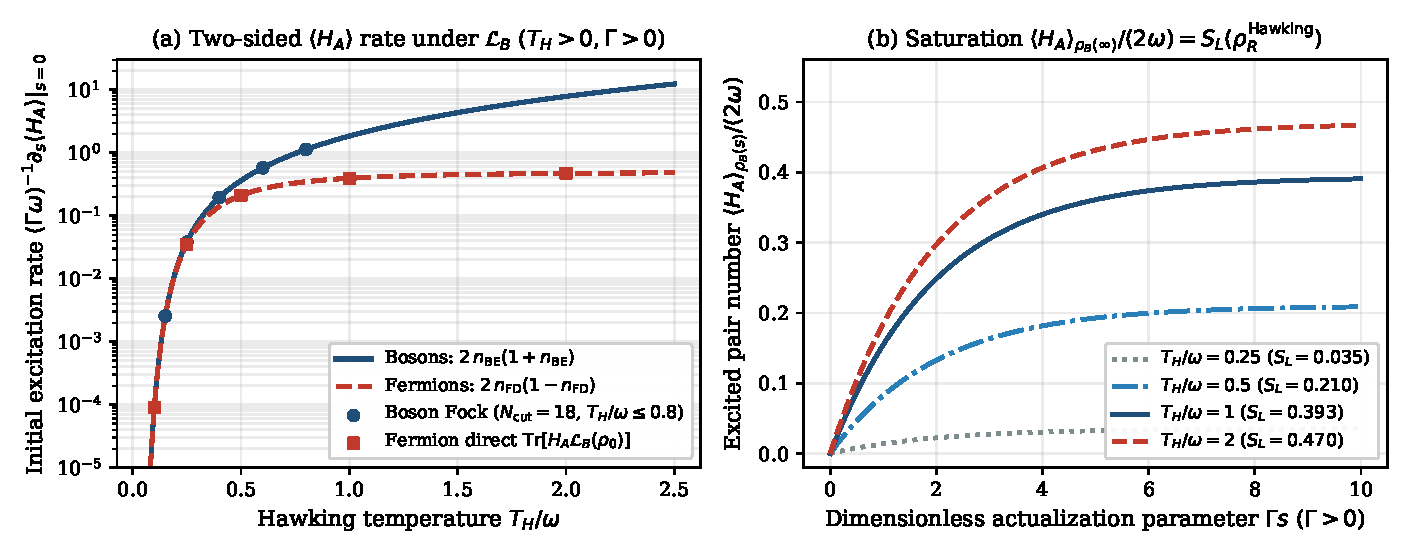
\includegraphics[width=\linewidth]{figures/fig1_horizon_heating.pdf}
  \caption{Two-sided inertial observable excitation when $B$'s exterior-local Killing-conserving flow $\cL_B(\rho) = -\frac{\Gamma}{2}[N_R,[N_R,\rho]]$ ($\Gamma>0$) acts on $|0_A\rangle$ (Theorem~\ref{thm:horizon}(f) and Eq.~\eqref{eq:unified-heating}; both one-sided reduced states $\Tr_L\rho_B(s)$ and $\Tr_R\rho_B(s)$ remain invariant). (a)~Exact analytic curves of the initial two-sided excitation rate vs.\ $T_H/\omega$, overlaid with truncated bosonic Fock checks ($N_{\mathrm{cut}}=18$, $T_H/\omega\le 0.8$, max rel.\ error $7.58\times 10^{-9}$) and independent direct fermionic matrix evaluations $\Tr[H_A\cL_B(\rho_0)]$. (b)~Auxiliary-time saturation ($s\ge 0$) of the excited fermionic pair number $\langle H_A\rangle_{\rho_B(s)}/(2\omega)$ to the constant linear Hawking entropy $S_L(\rho_R^{\mathrm{Hawking}})$ \eqref{eq:firewall-entropy}.}
  \label{fig:heating}
\end{figure}

\begin{remark}[Physical scope: reduced states, eigenbasis average vs.\ vacuum excitation, phase-noise equivalence, and terrestrial tests]\label{rem:horizon-scope}
Four structural caveats delineate the exact physical reach of Theorem~\ref{thm:horizon}:
\begin{enumerate}
  \item \emph{Two-sided observable vs.\ invariant one-sided reduced states:} Throughout the evolution \eqref{eq:ferm-energy-s}, the exterior reduced state $\Tr_L\rho_B(s) = (1-n_{\mathrm{FD}})|0\rangle\langle 0| + n_{\mathrm{FD}}|1\rangle\langle 1|$ is strictly constant (so $S_L(\rho_R^{\mathrm{Hawking}})$ in \eqref{eq:firewall-entropy} is a fixed initial property of $|0_A\rangle$ quantifying the destroyed cross-horizon coherence), and by exterior locality plus trace preservation ($\cL_B^\dagger(\1)=0$) the interior reduced state $\Tr_R\rho_B(s)$ is likewise invariant for \emph{every} initial state (\code{fermionic\_\allowbreak hawking\_\allowbreak reduced\_\allowbreak states\_\allowbreak invariant}). Along this trajectory starting from $|0_A\rangle$, only two-sided observables coupling $R$ and $L$ (such as $H_A$) detect the channel (left-marginal invariance holds for every input, while right-marginal invariance relies on the initial right reduced state commuting with $N_R$).
  \item \emph{Eigenbasis average vs.\ ground-state excitation (explicit counterexample):} Equation~\eqref{eq:heating-bound} bounds the \emph{eigenbasis average} over all eigenstates of $H_A$, and $\gamma_{\mathrm{loc}}>0$ alone does \emph{not} imply excitation of the ground state. Explicitly, on $\bbC^4$ take $H_B = N_R + N_L$, $\cA_B = M_2(\bbC)_R\otimes\1_L$, $L = N_R$, and $H_A = \mathrm{diag}(0,2,2,3) + |01\rangle\langle 10| + |10\rangle\langle 01|$. Then $[H_A,H_B]=0$, $H_A\succeq 0$ has unique $E=0$ ground state $|00\rangle$, the unique traceless direction in $\cA_B\cap\{H_B\}'$ is $N_R-\frac{1}{2}\1_4$ giving $\gamma_{\mathrm{loc}} = 2 > 0$, and the eigenbasis-averaged initial variance rate is $\frac{1}{4}\Tr\Gamma_{\cL}(H_A,H_A) = \frac{1}{2} > 0$. Nevertheless, $\cL(|00\rangle\langle 00|) = 0$, so both mean-energy and variance drift vanish identically on $|00\rangle$ (formalized as \code{positive\_\allowbreak gamma\_\allowbreak loc\_\allowbreak fixed\_\allowbreak ground\_\allowbreak state\_\allowbreak counterexample}). Thus the vacuum excitation in Theorem~\ref{thm:horizon}(f) requires the specific entangled structure of $|0_A\rangle$ and jump $N_R$, not $\gamma_{\mathrm{loc}}>0$ alone.
  \item \emph{Operational phase-noise equivalence and continuum requirements:} The single-mode channel $\Phi_B(s)$ is identical to averaging the random exterior phase unitary $e^{-i\theta N_R}$ over $\theta\sim\mathcal{N}(0,\Gamma s)$ (verified to $8.44\times 10^{-17}$ in Section~\ref{sec:matrix}) and can therefore be realized equally by ordinary stochastic phase noise or unitary coupling to an external environment. Existing QFT studies analyze the relation between accelerated Rindler-particle absorption and inertial particle creation in concrete detector-field coupling models \cite{UnruhWald1984} and derive Killing-horizon decoherence from soft radiation \cite{DSW2023}. Our result isolates the mode-level algebra of the chosen non-selective local channel; claiming a genuinely gravitational heating signature beyond unitary environmental decoherence requires specifying normalized wavepackets, detector-field coupling, a physical mapping $s(\tau)$, renormalized continuum stress-energy $\langle T_{\mu\nu}\rangle$, Hadamard regularity, and at least one observable separating it from standard unitary environment models.
  \item \emph{Static proportional redshift ($\gamma_{\mathrm{loc}}=0$) does NOT automatically guarantee terrestrial null tests:} Theorem~\ref{thm:horizon}(c) proves only that proportional clocks ($H_B = \alpha H_A$) create \emph{zero inter-observer clock incompatibility} ($\gamma_{\mathrm{loc}} = 0$). For Hermitian-jump (unital) flows, it does \emph{not} imply zero dephasing of observables outside the commutant fixed-point algebra $\cF_O = \{L_{O,k}\}'$. (Note that for general non-unital GKSL generators, expectation-value conservation $\cL^\dagger(M)=0$ need not coincide with $\{L_{O,k}\}'$: e.g., $H=\mathrm{diag}(0,0,0,1)$, $L_0=|0\rangle\langle 2|$, $L_1=|1\rangle\langle 2|$, $M=\mathrm{diag}(1,-1,0,0)$ satisfies $\cL^\dagger(H)=\cL^\dagger(H^2)=\cL^\dagger(M)=0$ while $\normF{[M,L_k]}=1$ and $\cL^\dagger(M^2)=2|2\rangle\langle 2|\neq 0$.) Explicitly, take $H_A = \frac{1}{2}\sigma_z$, $H_B = 2H_A$, $L = \sqrt{\Gamma}H_A$, and $\rho_0 = |+\rangle\langle +|$: here $\gamma = 0$ and all moments of $H_A$ and $H_B$ are strictly conserved, yet the interferometric observable $\sigma_x \notin \{H_A\}'$ decays exponentially as $\langle\sigma_x\rangle_s = e^{-\Gamma s/2}$ (at $\Gamma=1, s=2$: $\langle\sigma_x\rangle = e^{-1} \approx 0.3679$, purity $\Tr(\rho_s^2) = \frac{1+e^{-2}}{2} \approx 0.5677$). Linking Eq.~\eqref{eq:unified-heating} or laboratory dephasing to physical proper time $\tau$ requires specifying the jump operators, their normalization, target degrees of freedom, signal coupling, and $s(\tau)$, yielding $\Gamma_{\mathrm{eff}}(\tau) = \Gamma_O\,\frac{ds}{d\tau}$ (giving visibility $\mathcal{V}(\tau) = \exp[-\frac{1}{2}\int_0^\tau \Gamma_{\mathrm{eff}}(u)\,du]$ in the qubit model). Consequently, precision equivalence-principle measurements (MICROSCOPE \cite{MICROSCOPE2022}) and macroscopic matter-wave interferometry (Pedalino et al.\ \cite{Pedalino2025}) are not predicted parameter-free by $\gamma_{\mathrm{loc}}=0$, but constrain $\Gamma_{\mathrm{eff}}(\tau)$ once a concrete coupling is specified.
\end{enumerate}
\end{remark}

%==============================================================================
\section{Joint-Extension Monogamy vs.\ Observer Separation}\label{sec:cpl}
%==============================================================================

If observers $A$ and $B$ carry observer-separated CPTP channels $(\cE_A, \cE_B)$ (for example, reversible clock-time encodings $\cE_O = \cU_O(t)$ in Theorem~\ref{thm:cpl}(d) below, or composite two-time evolutions $\Phi_O(s)\circ\cU_O(t)$ combining Definition~\ref{def:ostqd}'s reversible flow with its auxiliary-time semigroup $\Phi_O(s) = e^{s\cL_O}$), what consistency condition links their predictions on causally shared observables? Inspired by Adlam and Rovelli's Cross-Perspective Links (CPL) \cite[Def.~4.1]{AdlamRovelli2022}, we first formulate \emph{marginal-state Cross-Perspective Consistency} on a chosen shared observable subalgebra $\cA_{\mathrm{sh}}$ (embedded via $j_A: \cA_{\mathrm{sh}} \to \cA_A$ and $j_B: \cA_{\mathrm{sh}} \to \cA_B$):
\begin{equation}\label{eq:cpl}
  \Tr\bigl(j_A(X)\,\cE_A(\rho)\bigr) = \Tr\bigl(j_B(X)\,\cE_B(\rho)\bigr) \qquad \forall X \in \cA_{\mathrm{sh}},\;\forall \rho.
\end{equation}
Equation~\eqref{eq:cpl} guarantees equality of all single-measurement marginal distributions on $\cA_{\mathrm{sh}}$; as shown in Remark~\ref{rem:cpl-wigner}, single-trial record agreement additionally requires specifying selective quantum instruments and their causal composition (constructed explicitly in Theorem~\ref{thm:cpl}(e)).
When $A$ and $B$ share a \emph{common causal future} in which both bring decoded copies $A'$ and $B'$ of an unknown logical system $C$ (dimension $d_C \ge 2$, maximally entangled with a reference $R$ in $|\Phi_{d_C}\rangle_{RC} = d_C^{-1/2}\sum_{i=0}^{d_C-1} |i\rangle_R |i\rangle_C$) into one joint laboratory, quantum mechanics requires a single normalized joint Choi state $\sigma_{RA'B'} \in \cD((\bbC^{d_C})^{\otimes 3})$ satisfying the CPTP marginal constraint $\Tr_{A'B'}(\sigma_{RA'B'}) = \1_R / d_C$. Define the Bell-overlap projections
\begin{equation}
  P_A := |\Phi_{d_C}\rangle\langle\Phi_{d_C}|_{RA'} \otimes \1_{B'}, \qquad
  P_B := |\Phi_{d_C}\rangle\langle\Phi_{d_C}|_{RB'} \otimes \1_{A'},
\end{equation}
so that the two observers' Schumacher entanglement fidelities \cite{Schumacher1996} are $F_A(\sigma) := \Tr(P_A\sigma)$ and $F_B(\sigma) := \Tr(P_B\sigma)$.

\begin{theorem}[Joint-Extension Band, Asymmetric Choi Saturation, Separate-Condition Reversible CPL, and Causal Shared-Record Instrument]\label{thm:cpl}
Let $d_C \ge 1$ (note that $d_C = 1$ is the trivial case in which all fidelities equal $1$; nontrivial strict tradeoffs and non-unit ceilings hold for $d_C \ge 2$).
\begin{enumerate}
  \item[(a)] \emph{(Exact projection overlap algebra)} $P_A$ and $P_B$ are Hermitian projections ($P_A^\dagger = P_A = P_A^2$, $P_B^\dagger = P_B = P_B^2$) obeying
  \begin{equation}\label{eq:papbpa}
    P_A P_B P_A = \frac{1}{d_C^2}\, P_A, \qquad P_B P_A P_B = \frac{1}{d_C^2}\, P_B.
  \end{equation}
  \item[(b)] \emph{(Sharp linear outer envelope and valid CPTP Choi saturation witness)} For every normalized pure state $|\psi\rangle \in (\bbC^{d_C})^{\otimes 3}$ and every convex mixture $\sigma_{RA'B'} = \sum_k w_k |\psi_k\rangle\langle\psi_k|$ ($w_k \ge 0$, $\sum_k w_k = 1$),
  \begin{equation}\label{eq:joint-bound}
    F_A(\sigma) + F_B(\sigma) \;\le\; 1 + \frac{1}{d_C}.
  \end{equation}
  In particular, for every $d_C \ge 2$, no joint CPTP extension supports $F_A = F_B = 1$. Moreover, the linear sum bound \eqref{eq:joint-bound} is sharp even under the CPTP Choi marginal constraint $\Tr_{A'B'}(\sigma_*) = \1_R / d_C$: it is attained symmetrically by the mixed Choi state
  \begin{equation}\label{eq:choi-witness}
    \sigma_* := \frac{1}{d_C}\sum_{j=0}^{d_C-1} |\psi_j\rangle\langle\psi_j|, \qquad
    |\psi_j\rangle := \frac{|\Phi_{d_C}\rangle_{RA'}|j\rangle_{B'} + |\Phi_{d_C}\rangle_{RB'}|j\rangle_{A'}}{\sqrt{2 + 2/d_C}},
  \end{equation}
  which satisfies $\Tr_{A'B'}(\sigma_*) = \1_R / d_C$ and $F_A(\sigma_*) = F_B(\sigma_*) = \frac{1 + 1/d_C}{2}$. (By contrast, the naive product state $|\Phi_{d_C}\rangle_{RA'}\otimes |0\rangle_{B'}$ attains only $(F_A, F_B) = (1, 1/d_C^2)$, strictly below the linear envelope for all $d_C \ge 2$.)
  \item[(c)] \emph{(Complete achievable joint region: curved upper/lower boundaries \cite{Kay2009,Nechita2021} and constructive CPTP Choi attainment)} For $d_C \ge 2$, let $a := 1/d_C$ and $b := \sqrt{1 - a^2}$. The linear inequality \eqref{eq:joint-bound} is a sharp \emph{outer sum envelope}, not the full achievable $(F_A, F_B)$ region: every joint state $\sigma_{RA'B'}$ obeys both the concave curved upper tradeoff \cite[Eq.~(6)]{Kay2009} and the reverse-triangle-inequality lower bound
  \begin{equation}\label{eq:kay-curved}
    F_B^{\min}(F_A) := \Bigl[\max\!\Bigl(0,\; a\sqrt{F_A} - b\sqrt{1 - F_A}\Bigr)\Bigr]^2
    \;\le\; F_B \;\le\;
    \Bigl(a\sqrt{F_A} + b\sqrt{1 - F_A}\Bigr)^2 =: F_B^{\max}(F_A).
  \end{equation}
  For $d_C \ge 2$, the upper curve lies strictly below the tangent $F_A + F_B = 1 + 1/d_C$ everywhere except the symmetric contact point $F_A = F_B = (1+1/d_C)/2$, and both curves converge to $F_B = 1/d_C^2$ at $F_A = 1$ (e.g.\ at $d_C = 2$ and $F_A = 0.9$, $F_B^{\min} = \frac{6-3\sqrt{3}}{20} \approx 0.0402 \le F_B \le \frac{6+3\sqrt{3}}{20} \approx 0.5598$, strictly tighter than $1.5 - 0.9 = 0.6$). Moreover, the \emph{entire} shaded band \eqref{eq:kay-curved} is attained by valid CPTP Choi states ($\Tr_{A'B'}\sigma = \1_R/d_C$): defining $u_j := |\Phi_{d_C}\rangle_{RA'}|j\rangle_{B'}$, $v_j := |\Phi_{d_C}\rangle_{RB'}|j\rangle_{A'}$, $w_j := (v_j - a u_j)/b$, and $|\psi_j^\pm(x)\rangle := \sqrt{x}\,u_j \pm \sqrt{1-x}\,w_j$, the equal-weight mixtures
  \begin{equation}\label{eq:asym-choi}
    \sigma^\pm(x) := \frac{1}{d_C}\sum_{j=0}^{d_C-1} |\psi_j^\pm(x)\rangle\langle\psi_j^\pm(x)|
  \end{equation}
  satisfy $\Tr_{A'B'}\sigma^\pm(x) = \1_R/d_C$: $\sigma^+(x)$ attains the full upper boundary $(x, F_B^{\max}(x))$ for all $x\in[0,1]$ (reducing to \eqref{eq:choi-witness} at $x=(1+a)/2$), and $\sigma^-(x)$ attains the curved lower boundary $(x, F_B^{\min}(x))$ for all $x\in[b^2,1]$ (including $(b^2,0)$). For the flat lower boundary $0\le x\le b^2$ ($F_B=0$), the shift measure-and-prepare channel measuring computational basis $|j\rangle$ and preparing $|j+1\bmod d_C\rangle$ on both outputs has Choi state $\sigma^{(0,0)}$ attaining $(0,0)$, so $(1-x/b^2)\sigma^{(0,0)} + (x/b^2)\sigma^-(b^2)$ attains $(x,0)$. Finally, convex combinations $\lambda\sigma^+(x) + (1-\lambda)\sigma_{\min}(x)$ ($\lambda\in[0,1]$) attain every interior point $(x,y)$ with $F_B^{\min}(x)\le y\le F_B^{\max}(x)$. (Note the distinction in prior literature: Kay, Kaszlikowski, and Ramanathan \cite[Eq.~(6), Fig.~1]{Kay2009} maximize the singlet fraction over local unitaries, whereas our fixed-Bell overlaps $(F_A,F_B)$ can vanish and correspond directly to the full universal asymmetric cloning region of Nechita, Pellegrini, and Rochette \cite[\S 7, Theorem~6, Fig.~2]{Nechita2021} via $F_i = p_i + (1-p_i)/d_C^2$ for depolarizing marginals $T_i(\rho) = p_i\rho + (1-p_i)\1/d_C$, to which any joint Choi state maps under $\bar{U}\otimes U\otimes U$ twirling without changing $(F_A,F_B)$.)
  \item[(d)] \emph{(Constructive separate-condition reversible channels with marginal CPL on a shared factor commuting with logical operations)} On $\cH_C \otimes \cH_{\mathrm{sh}} \cong \bbC^{d_C} \otimes \bbC^m$, for any unitary $V_B \in U(d_C)$, define the separate-condition reversible channels $\cE_A(\rho) = \rho$ and $\cE_B(\rho) = (V_B\otimes\1_{\mathrm{sh}})\rho(V_B\otimes\1_{\mathrm{sh}})^\dagger$, with explicit decoders $\cR_A = \id$ and $\cR_B(\sigma) = (V_B^\dagger\otimes\1_{\mathrm{sh}})\sigma(V_B\otimes\1_{\mathrm{sh}})$. Under these two separate experimental conditions, each decoder attains $F_e(\cR_A\circ\cE_A) = 1$ and $F_e(\cR_B\circ\cE_B) = |\Tr(V_B^\dagger V_B)|^2/d_C^2 = 1$ (without $\cR_B$, $F_e(\mathrm{Ad}_{V_B}) = |\Tr V_B|^2/d_C^2$ can vanish, e.g.\ $0$ for $V_B = \sigma_z$), while exact marginal-state CPL \eqref{eq:cpl} holds on the shared tensor factor $\cA_{\mathrm{sh}} = \1_C \otimes M_m(\bbC)$ commuting with the logical operations on $\cH_C$ (non-commutative for $m > 1$; restricting to classical records selects a commutative diagonal subalgebra $\1_C\otimes D_m \subset \cA_{\mathrm{sh}}$).
  \item[(e)] \emph{(Causal shared-record projective readout composed with record-preserving propagation)} On $\cH_C \otimes \cH_{\mathrm{rec}} \cong \bbC^{d_C}\otimes\bbC^m$ with commutative classical-record subalgebra $\cA_{\mathrm{rec}} = \1_C\otimes D_m$ ($D_m$ diagonal in $\{|x\rangle_{\mathrm{rec}}\}_{x=0}^{m-1}$), let observer $A$ apply record-preserving logical propagation $U_A\in U(d_C)$ composed with an \emph{ideal projective record readout} $\cI_{A,x}(\rho) := K_{A,x}\rho K_{A,x}^\dagger$, $K_{A,x} := U_A \otimes |x\rangle\langle x|_{\mathrm{rec}}$, followed causally downstream in a shared future region by observer $B$'s ideal projective readout $\cI_{B,y}(\sigma) := K_{B,y}\sigma K_{B,y}^\dagger$, $K_{B,y} := U_B \otimes |y\rangle\langle y|_{\mathrm{rec}}$ ($U_B\in U(d_C)$). Then for every prepared state $\rho$:
  \begin{enumerate}
    \item[(i)] $\{\cI_{A,x}\}$, $\{\cI_{B,y}\}$, and the causal sequential composition $\{\cI_{B,y}\circ\cI_{A,x}\}$ are completely positive instruments summing to the projective pinching maps $\sum_x \cI_{A,x} = \mathrm{Ad}_{U_A}\otimes\cP_{\mathrm{rec}}$ and $\sum_y \cI_{B,y} = \mathrm{Ad}_{U_B}\otimes\cP_{\mathrm{rec}}$ ($\sum_x K_{A,x}^\dagger K_{A,x} = \sum_y K_{B,y}^\dagger K_{B,y} = \1$). Up to the known logical unitary $U_A$, $\cP_{\mathrm{rec}}$ coincides with the $s\to\infty$ limit of record-basis dephasing (and matches finite-$s$ record dephasing on initially diagonal record states), whereas for $m\ge 2$ it differs on off-diagonal record coherences from any invertible finite-$s$ semigroup $e^{s\cL}$ (Remark~\ref{rem:def-precisions}(4) and Remark~\ref{rem:cpl-wigner}(1));
    \item[(ii)] joint single-trial outcome probabilities $P(x,y) := \Tr\bigl((\cI_{B,y}\circ\cI_{A,x})(\rho)\bigr)$ equal $\delta_{xy}\Tr\bigl((\1_C\otimes |x\rangle\langle x|)\rho\bigr)$, so single-trial record disagreement vanishes identically ($P(x\neq y) = 0$);
    \item[(iii)] local marginal expectations on $\cA_{\mathrm{rec}}$ agree identically between $A$, $B$, and the initial preparation: $\sum_x \cI_{A,x}^\dagger(\1_C\otimes D) = \1_C\otimes D = \sum_y \cI_{B,y}^\dagger(\1_C\otimes D)$ for all $D\in D_m$.
  \end{enumerate}
\end{enumerate}
\end{theorem}

\begin{proof}
(a) Direct index contraction on $(\mathrm{Fin}\,d_C)^3$ verifies \eqref{eq:papbpa} entrywise: $(P_A P_B P_A)_{(r,a,b),(r',a',b')} = \allowbreak d_C^{-2}(P_A)_{(r,a,b),(r',a',b')}$.
(b) For pure $|\psi\rangle$, let $u := P_A\psi$ and $w := P_B\psi$, so $\|u\|^2 = F_A$, $\|w\|^2 = F_B$, and $\|P_B u\|^2 = \langle\psi, P_A P_B P_A\psi\rangle = d_C^{-2}\|u\|^2$. Cauchy--Schwarz yields $|\mathrm{Re}\langle u,w\rangle| = |\mathrm{Re}\langle P_B u, w\rangle| \le d_C^{-1}\|u\|\,\|w\|$, so $\|u+w\|^2 \le (1+d_C^{-1})(\|u\|^2+\|w\|^2)$. Meanwhile $\|u\|^2+\|w\|^2 = \mathrm{Re}\langle\psi,u+w\rangle \le \|\psi\|\,\|u+w\|$, proving $F_A+F_B \le 1 + 1/d_C$; convex combinations extend this to all density matrices. For $\sigma_*$ in \eqref{eq:choi-witness}, direct summation verifies $\|\psi_j\|^2 = 1$, $F_A(\sigma_*)=F_B(\sigma_*)=(1+1/d_C)/2$, and $\Tr_{A'B'}\sigma_* = \1_R/d_C$.
(c) For any density matrix $\sigma \succeq 0$ ($\Tr\sigma=1$), write $S := \sqrt{\sigma}$, so $\sqrt{F_A} = \normF{P_A S}$, $\sqrt{1-F_A} = \normF{(\1-P_A)S}$, and $\sqrt{F_B} = \normF{P_B S}$. Using \eqref{eq:papbpa}, $\normF{P_B P_A S} = a\normF{P_A S} = a\sqrt{F_A}$, while $\normF{P_B(\1-P_A)S}^2 = \allowbreak \Tr\bigl(S(\1-P_A)P_B(\1-P_A)S\bigr) \le \allowbreak b^2\normF{(\1-P_A)S}^2 = b^2(1-F_A)$ because $(\1-P_A)P_B(\1-P_A)$ has nonzero eigenvalues equal to $1 - a^2 = b^2$. Applying the triangle and reverse-triangle inequalities to $P_B S = P_B P_A S + P_B(\1-P_A)S$ yields $\max(0, a\sqrt{F_A} - b\sqrt{1-F_A}) \le \allowbreak \sqrt{F_B} \le \allowbreak a\sqrt{F_A} + b\sqrt{1-F_A}$, proving both bounds in \eqref{eq:kay-curved} directly for arbitrary mixed states \cite{Kay2009,Nechita2021}. For $\sigma^\pm(x)$ in \eqref{eq:asym-choi}, orthonormality $\langle u_j, u_j\rangle = \langle w_j, w_j\rangle = 1$, $\langle u_j, w_j\rangle = 0$ gives $\|\psi_j^\pm(x)\|^2=1$, $P_A\psi_j^\pm(x) = \sqrt{x}\,u_j$, $P_B\psi_j^\pm(x) = (a\sqrt{x}\pm b\sqrt{1-x})v_j$, and summing over $j,a',b'$ cancels the cross-term partial trace so $\Tr_{A'B'}\sigma^\pm(x) = \1_R/d_C$. For the shift channel $\sigma^{(0,0)} = \frac{1}{d_C}\sum_j |j,j+1,j+1\rangle\langle j,j+1,j+1|$ (indices mod~$d_C$), $j+1\not\equiv j\pmod{d_C}$ for $d_C\ge 2$ implies $P_A\sigma^{(0,0)}=P_B\sigma^{(0,0)}=0$ and $\Tr_{A'B'}\sigma^{(0,0)}=\1_R/d_C$. Convex mixtures of $\sigma^{(0,0)}$ with $\sigma^-(b^2)$ attain $(x,0)$ for $x\in[0,b^2]$, and convex mixtures of $\sigma^+(x)$ with the lower boundary $\sigma_{\min}(x)$ preserve $\Tr_{A'B'}(\cdot)=\1_R/d_C$ and attain every $y\in[F_B^{\min}(x),F_B^{\max}(x)]$.
(d) Unitarity of $V_B$ gives $(V_B\otimes\1_{\mathrm{sh}})^\dagger(\1_C\otimes X_{\mathrm{sh}})(V_B\otimes\1_{\mathrm{sh}}) = \1_C\otimes X_{\mathrm{sh}}$ and $|\Tr(V_B^\dagger V_B)|^2/d_C^2 = 1$.
(e) Orthogonality $|y\rangle\langle y|\,|x\rangle\langle x| = \delta_{xy}|x\rangle\langle x|$ gives $K_{B,y}K_{A,x} = \delta_{xy}(U_B U_A)\otimes |x\rangle\langle x|$, from which (i)--(iii) follow directly by trace cyclicity and unitarity of $U_A, U_B$. Parts (a), (b) (pure, mixed, and $\sigma_*$), complete shaded-region CPTP Choi achievability of (c) (\code{asymmetric\_\allowbreak kay\_\allowbreak choi\_\allowbreak saturation} and \code{achievable\_\allowbreak joint\_\allowbreak region\_\allowbreak choi\_\allowbreak complete}), (d), (e), and the finite-$s$ weak-measurement contrast (\code{weak\_\allowbreak record\_\allowbreak measurement\_\allowbreak vs\_\allowbreak projective\_\allowbreak readout}) are machine-checked in \code{OSTQD/\allowbreak Theorem3\_\allowbreak CrossPerspective.lean}; the curved inequalities \eqref{eq:kay-curved} and operational Choi correspondence are hand-proved and audited numerically (Table~\ref{tab:lean}).
\end{proof}

\begin{remark}[Scope of Theorem~\ref{thm:cpl}(d)--(e), finite-$s$ weak readout contrast, causal asymmetry, and Wigner's friend no-go theorems]\label{rem:cpl-wigner}
Four structural caveats govern the physical interpretation of Theorem~\ref{thm:cpl}:
\begin{enumerate}
  \item \emph{Marginal consistency, ideal projective readout ($s\to\infty$), and finite-$s$ weak measurements:} Equation~\eqref{eq:cpl} ensures only agreement of single-measurement marginals on $\cA_{\mathrm{sh}}$, which is strictly weaker than Adlam and Rovelli's single-trial CPL \cite[Def.~4.1]{AdlamRovelli2022}: the correlated state $\rho_{\mathrm{corr}} = \frac{1}{2}(|00\rangle\langle 00| + |11\rangle\langle 11|)$ and the maximally mixed state $\rho_{\mathrm{ind}} = \1_4/4$ share identical single-bit marginals yet have single-trial disagreement probabilities $0$ and $1/2$, respectively. Theorem~\ref{thm:cpl}(e) attains $P(x\neq y)=0$ via an \emph{ideal projective readout} composed after record-preserving propagation (whose non-selective sum $\mathrm{Ad}_{U_A}\otimes\cP_{\mathrm{rec}}$ matches record dephasing in the $s\to\infty$ limit or on already-diagonal record states, not an invertible finite-$s$ semigroup $e^{s\cL}$ on the full algebra). To match a finite-$s$ qubit $Z$-record dephasing map $\Phi(s)$ non-selectively on all states, one instead uses weak-measurement Kraus operators $M_\pm = \sqrt{(\1\pm\eta Z)/2}$ with $\sqrt{1-\eta^2} = e^{-\Gamma s/2}$; two consecutive identical weak measurements then disagree with universal probability $(1-\eta^2)/2 = \frac{1}{2}e^{-\Gamma s}$ for every input state (decreasing from $1/2$ at $\Gamma s=0$ to $0$ in the $s\to\infty$ projective limit, e.g.\ $0.1839397$ at $\Gamma s = 1$, formalized in \code{weak\_\allowbreak record\_\allowbreak measurement\_\allowbreak vs\_\allowbreak projective\_\allowbreak readout}; by contrast, randomly applying $\1$ or $Z$ with probabilities $(1\pm e^{-\Gamma s/2})/2$ and reporting which operator was applied yields a distinct operator-label disagreement rate $\frac{1}{2}(1-e^{-\Gamma s})$), demonstrating that single-trial agreement depends on specifying the readout instrument as well as the channel. Figure~\ref{fig:joint-bottleneck}(a) explicitly labels $(1,1)$ as a \emph{separate-condition} decoding point rather than a joint two-output channel.
  \item \emph{Asymmetry of the causal-future condition and AMPS composition rules:} The existence of a common causal future in which both decoded copies are brought together \emph{implies} the existence of a single joint two-output channel $\Psi_{AB}$ and hence \eqref{eq:joint-bound}--\eqref{eq:kay-curved}. However, the \emph{converse does not hold automatically} without an additional physical postulate: two observers who never meet in the future can still receive halves of a pre-prepared bipartite state described by a single joint state/channel. Consequently, connecting to the AMPS scenario \cite[\S 2]{AMPS2013}---in particular, an observer who collects early Hawking radiation records and carries them across the horizon---requires specifying explicitly which operational subsets of interventions can be composed in a single experiment alongside no-signaling and record-merging rules \cite{HausmannRenner2025,Walleghem2025,Adlam2026}.
  \item \emph{Physical identification of $\cA_{\mathrm{sh}}$ and integration with $s$-flows:} Showing that pre-horizon, ADM, or early-radiation records lie inside a commuting shared factor $\cA_{\mathrm{sh}}$ (or $\cA_{\mathrm{rec}}$) is a modeling assumption, not proved from general relativity here. Integrating Theorem~\ref{thm:cpl}(d) with irreversible $s$-actualization is achieved via the finite-width decoherence-free energy window of Theorem~\ref{thm:double}(f) (realized in Section~\ref{sec:matrix}).
  \item \emph{Relation to extended Wigner's friend no-go theorems:} Relative to \cite{FrauchigerRenner2018,Bong2020,HausmannRenner2025,Walleghem2025,Adlam2026}, OSTQD does \emph{not} claim to retain all standard assumptions simultaneously: it retains unitary $t$-evolution within each observer's perspective, marginal CPL \eqref{eq:cpl} on $\cA_{\mathrm{sh}}$, and single-trial record agreement on causally accessible classical records (Theorem~\ref{thm:cpl}(e)), while relaxing observer-independent absoluteness of uncompared quantum facts when no joint operational composition is specified. Whether dynamical complexity (such as Harlow--Hayden \cite{HarlowHayden2013}) prevents operational violation of \eqref{eq:kay-curved} in every gravitational initial state remains an open question beyond our finite-dimensional theorem.
\end{enumerate}
\end{remark}

%==============================================================================
\section{Parisi--Wu Arrow, Spectral Pinching, Energy Windows, and Dimension Bottlenecks}\label{sec:double-bottleneck}
%==============================================================================

We next formalize the directed monotonicity of Hermitian-jump $s$-flows, establish the exact connection between $\lim_{s\to\infty} e^{s\cL}$ and orthogonal pinching $\cP$, clarify the algebraic double-uncertainty decomposition relative to Baumgratz--Cramer--Plenio \cite{Baumgratz2014} and Lidar--Chuang--Whaley \cite{Lidar1998}, resolve the exact-eigenspace scrambling obstruction via finite-width energy windows, and state the sharp intermediate-dimension bottleneck bound.

Let $\{K_k\}_{k=1}^m$ be Hermitian jump operators ($K_k^\dagger = K_k$) generating the unital actualization flow $\cL(\rho) = -\frac{1}{2}\sum_k [K_k, [K_k, \rho]]$. Denote the \emph{linear entropy} by $S_L(\rho) := 1 - \Tr(\rho^2)$ (distinct from the R\'enyi-2 entropy $S_2(\rho) := -\ln\Tr(\rho^2)$, although both are monotone functions of purity), and let $\cP(\rho) := \sum_{\alpha=1}^r \Pi_\alpha \rho \Pi_\alpha$ be the orthogonal pinching map associated with a complete family of orthogonal projections ($\Pi_\alpha^\dagger = \Pi_\alpha = \Pi_\alpha^2$, $\Pi_\alpha\Pi_\beta = \delta_{\alpha\beta}\Pi_\alpha$, $\sum_\alpha \Pi_\alpha = \1$).

\begin{theorem}[Parisi--Wu Purity Arrow, Spectral Block Decay, Pinching Identity, and Finite-Width Energy Windows]\label{thm:double}
For every Hermitian matrix $\rho = \rho^\dagger \in M_d(\bbC)$ (and, where von Neumann entropy is stated, every density matrix $\rho \succeq 0$ with $\Tr\rho = 1$):
\begin{enumerate}
  \item[(a)] \emph{(Directed Parisi--Wu purity arrow)}
  \begin{equation}\label{eq:pw-arrow}
    \left.\frac{\partial}{\partial s}\,\Tr\bigl(\rho(s)^2\bigr)\right|_{s=0} = 2\Tr\bigl(\rho\,\cL(\rho)\bigr) = -\sum_k \normF{[K_k, \rho]}^2 \;\le\; 0,
  \end{equation}
  with equality iff $[K_k, \rho] = 0$ for all $k$ (strict decrease outside the fixed-point algebra $\cF = \{K_k\}'$).
  \item[(b)] \emph{(Exact linear-entropy Pythagorean identity)} For any orthogonal pinching $\cP$ and any Hermitian $\rho$,
  \begin{equation}\label{eq:pythagorean}
    S_L\bigl(\cP(\rho)\bigr) \;=\; S_L(\rho) \;+\; \normF{\rho - \cP(\rho)}^2.
  \end{equation}
  For any density matrix $\rho \succeq 0$ ($\Tr\rho=1$), the von Neumann analogue is $S(\cP(\rho)) = S(\rho) + D(\rho \,\|\, \cP(\rho))$ \cite{Baumgratz2014}.
  \item[(c)] \emph{(Fixed-point observable invisibility)} Every observable $M \in \cF = \{K_k\}'$ satisfies $\cL^\dagger(M) = 0$, hence $\Tr(M\,e^{s\cL}(\rho)) = \Tr(M\rho)$ for all $s \ge 0$.
  \item[(d)] \emph{(Decoherence-free sector preservation \cite{Lidar1998})} If $\rho$ is supported inside a single sector $\Pi_\alpha$ ($\Pi_\alpha\rho\Pi_\alpha = \rho$) on which each $K_k$ acts as a scalar $c_{k,\alpha}\Pi_\alpha$, then $\cL(\rho) = 0$ and $\cP(\rho) = \rho$ identically.
  \item[(e)] \emph{(Spectral block decay linking $\lim_{s\to\infty} e^{s\cL} = \cP$)} Suppose the Hermitian jumps $\{K_k\}$ simultaneously act as scalars $\lambda_{k,\alpha} \in \bbR$ on each orthogonal sector $\Pi_\alpha$ ($K_k\Pi_\alpha = \Pi_\alpha K_k = \lambda_{k,\alpha}\Pi_\alpha$, i.e., commuting spectral jumps $K_k = \sum_\alpha \lambda_{k,\alpha}\Pi_\alpha$). Then every off-diagonal block $\Pi_\alpha\rho\Pi_\beta$ is an exact eigenvector of $\cL$:
  \begin{equation}\label{eq:block-eigen}
    \cL(\Pi_\alpha\rho\Pi_\beta) = -\frac{1}{2}\left(\sum_{k=1}^m (\lambda_{k,\alpha} - \lambda_{k,\beta})^2\right)\Pi_\alpha\rho\Pi_\beta.
  \end{equation}
  Consequently, $e^{s\cL}(\Pi_\alpha\rho\Pi_\beta) = \exp\!\bigl[-\frac{s}{2}\sum_k(\lambda_{k,\alpha}-\lambda_{k,\beta})^2\bigr]\Pi_\alpha\rho\Pi_\beta$. Whenever the eigenvalue tuples $(\lambda_{k,\alpha})_k$ separate distinct sectors ($\forall \alpha\neq\beta, \exists k, \lambda_{k,\alpha}\neq\lambda_{k,\beta}$), the exact long-time limit is $\lim_{s\to\infty} e^{s\cL}(\rho) = \cP(\rho)$, identifying $\normF{\rho-\cP(\rho)}^2$ in \eqref{eq:pythagorean} precisely with the coherence destroyed by the $s$-flow.
  \item[(f)] \emph{(Finite-width microcanonical energy-window compatibility with non-stationary $t$-evolution)} Let $H = H^\dagger$ commute with a coarse-grained window projector $\Pi_{\mathrm{win}} = \1_{[E-\Delta, E+\Delta]}(H)$ (so $H$ may be \emph{non-scalar} inside $\Pi_{\mathrm{win}}$), and let coarse-grained jump operators $\{K_k\}$ satisfy $[K_k, H] = 0$ and $K_k\Pi_{\mathrm{win}} = \Pi_{\mathrm{win}}K_k = c_k\Pi_{\mathrm{win}}$ (piecewise constant on the energy window). Then for every state $\rho$ supported in $\Pi_{\mathrm{win}}$,
  \begin{equation}\label{eq:window-compat}
    \cL(\rho) = 0, \qquad \cL([H,\rho]) = [H,\cL(\rho)] = 0, \qquad \Pi_{\mathrm{win}}(-i[H,\rho])\Pi_{\mathrm{win}} = -i[H,\rho],
  \end{equation}
  so non-stationary unitary $t$-evolution proceeds inside $\Pi_{\mathrm{win}}$ for any state with $[H,\rho] \neq 0$ (whereas eigenstates or functions $f(H)$ remain stationary), while the $s$-actualization flow leaves the entire window trajectory pointwise invariant.
\end{enumerate}
\end{theorem}

\begin{proof}
(a)--(d) follow from $[K,\rho]^\dagger = -[K,\rho]$, trace cyclicity, and $\Tr(\cP(\rho)\rho) = \Tr(\cP(\rho)^2)$.
(e) Using $K_k\Pi_\alpha = \lambda_{k,\alpha}\Pi_\alpha$ and $\Pi_\beta K_k = \lambda_{k,\beta}\Pi_\beta$, $[K_k, \Pi_\alpha\rho\Pi_\beta] = (\lambda_{k,\alpha}-\lambda_{k,\beta})\Pi_\alpha\rho\Pi_\beta$, and iterating the commutator gives $-\frac{1}{2}[K_k,[K_k,\Pi_\alpha\rho\Pi_\beta]] = -\frac{1}{2}(\lambda_{k,\alpha}-\lambda_{k,\beta})^2 \Pi_\alpha\rho\Pi_\beta$; summing over $k$ yields \eqref{eq:block-eigen} and its exact exponential.
(f) Applying (d) gives $\cL(\rho) = 0$; Theorem~\ref{thm:bps}(d) gives $\cL([H,\rho]) = [H,\cL(\rho)] = 0$; and $[H,\Pi_{\mathrm{win}}]=0$ with $\Pi_{\mathrm{win}}\rho\Pi_{\mathrm{win}}=\rho$ gives $\Pi_{\mathrm{win}}(-i[H,\rho])\Pi_{\mathrm{win}} = -i[H,\rho]$. All algebraic parts (a)--(f) are formalized in \code{OSTQD/Theorem4\_DoubleUncertainty.lean}.
\end{proof}

\begin{remark}[Relation to coherence theory, non-commuting jumps, and why exact single eigenspaces fail]\label{rem:coherence-window}
Three clarifications ensure strict alignment with quantum information theory:
(1)~When $\{K_k\}$ and $\cP$ are chosen independently without the spectral alignment of Theorem~\ref{thm:double}(e), $\cP$ need \emph{not} equal $\lim_{s\to\infty} e^{s\cL}$: for $K = \sigma_x$, $\rho = |+\rangle\langle +|$, and $\sigma_z$-pinching $\cP_z$, one has $e^{s\cL}(\rho) = \rho$ for all $s \ge 0$ while $\normF{\rho-\cP_z(\rho)}^2 = 1/2$. For general \emph{non-commuting} Hermitian jumps (such as $K_1=\sigma_x, K_2=\sigma_z$), $\cL$ is Hilbert--Schmidt self-adjoint and negative semidefinite with kernel $\cF = \{K_k\}'$, so $\lim_{s\to\infty} e^{s\cL}$ is the trace-preserving Hilbert--Schmidt orthogonal conditional expectation $E_{\cF}$ onto $\cF$ (here $E_{\cF}(\rho) = \frac{\Tr\rho}{2}\1_2$, which is not a simple block pinching), and the same Pythagorean identity $S_L(E_{\cF}(\rho)) = S_L(\rho) + \normF{\rho - E_{\cF}(\rho)}^2$ holds.
(2)~Following Baumgratz--Cramer--Plenio \cite{Baumgratz2014}, $S(\cP(\rho)) - S(\rho) = D(\rho\|\cP(\rho))$ is the standard relative entropy of coherence (generalized to block pinching), whereas the Hilbert--Schmidt quantity $\normF{\rho-\cP(\rho)}^2$ is a convenient $L^2$ algebraic measure rather than a universal coherence monotone under all incoherent operations. Furthermore, $S_L(\rho)$ is a function of the instantaneous state $\rho$ alone and cannot retrospectively distinguish environment entanglement from classical mixing without specifying the dynamical preparation.
(3)~In a \emph{single exact energy eigenspace} ($H_B\Pi_E = E\Pi_E$), $[H_B,\rho]=0$ identically, forbidding any nontrivial $t$-scrambling generated by $H_B$ itself! Theorem~\ref{thm:double}(f) resolves this constructively by replacing a single exact eigenvalue with a \emph{finite-width microcanonical window} $\Pi_{\mathrm{win}} = \1_{[E-\Delta, E+\Delta]}(H_B)$ on which coarse-grained $K_k = f_k(H_B)$ are piecewise constant. Note carefully that decoherence-free protection (as in Lidar--Chuang--Whaley \cite{Lidar1998}) guarantees that $s$-actualization does not \emph{destroy} unitary $t$-scrambling or radiation recovery; it is a compatibility condition rather than a standalone proof of fast scrambling or Page-curve recovery.
\end{remark}

\paragraph{Intermediate-dimension bottleneck bound (special case of Farber--Gour \cite{FarberGour2026}).}
Finally, consider any CPTP encoding channel $\cE: M_{d_C}(\bbC) \to M_{d_f}(\bbC)$ (Kraus operators $\{E_\alpha\}$, $\sum_\alpha E_\alpha^\dagger E_\alpha = \1_{d_C}$) passing through an intermediate Hilbert space $\cH_f \cong \bbC^{d_f}$, followed by any CPTP decoding channel $\cR: M_{d_f}(\bbC) \to M_{d_C}(\bbC)$ (Kraus operators $\{R_\beta\}$, $\sum_\beta R_\beta^\dagger R_\beta = \1_{d_f}$) \emph{without access to any classical side register or emitted radiation}. For an arbitrary input state $\rho$, Farber and Gour \cite{FarberGour2026} (\S IV, Theorem~5) proved that the optimal unassisted single-shot source fidelity (square root of entanglement fidelity) equals the Ky Fan $d_f$-norm $\|\rho\|_{(d_f)}$ (sum of the $d_f$ largest eigenvalues of $\rho$), attained by projecting onto the top eigenspace and resetting the complement. Specializing to the maximally mixed input $\rho = \1_{d_C}/d_C$ yields the squared-fidelity ceiling $\min(1, d_f^2/d_C^2)$ below; our contribution here is a self-contained elementary Kraus-operator proof, complete Lean~4 formalization across both $d_f\le d_C$ and $d_f > d_C$, an explicit classical-flag resource counterexample, and its conditional remnant interpretation.

\begin{theorem}[Intermediate-Dimension Bottleneck Bound on Entanglement Fidelity (Maximally Mixed Case of \cite{FarberGour2026})]\label{thm:bottleneck}
For all positive integers $d_C, d_f$ and all unassisted CPTP channels $\cE: M_{d_C}(\bbC) \to M_{d_f}(\bbC)$ and $\cR: M_{d_f}(\bbC) \to M_{d_C}(\bbC)$, the Schumacher entanglement fidelity \cite{Schumacher1996} on the maximally mixed input $\1_{d_C}/d_C$ obeys
\begin{equation}\label{eq:bottleneck}
  F_e(\cR \circ \cE) \;=\; \frac{1}{d_C^2}\sum_{\alpha,\beta}\bigl|\Tr(R_\beta E_\alpha)\bigr|^2 \;\le\; \min\!\left(1,\;\frac{d_f^2}{d_C^2}\right) \;=\; \min\!\left(1,\; e^{-2(S_C - S_f)}\right),
\end{equation}
where we define the mathematical log-dimensions $S_C := \ln d_C$ and $S_f := \ln d_f$ (in nats). Whenever $d_f \le d_C$, equality $F_e = d_f^2/d_C^2$ is attained by the CPTP encoder $E_0 = \sum_{a=0}^{d_f-1} |a\rangle_f\langle a|_C$ and complement-reset operators $E_j = |0\rangle_f\langle j|_C$ ($j = d_f,\dots,d_C-1$) with isometric decoder $R_0 = E_0^\dagger$. Whenever $d_f \ge d_C$, equality $F_e = 1$ is attained by the isometric encoder $E_0 = V = \sum_{i=0}^{d_C-1}|i\rangle_f\langle i|_C$ and reset decoder $R_0 = V^\dagger$, $R_k = |0\rangle_C\langle k|_f$ ($k = d_C,\dots,d_f-1$).
\end{theorem}

\begin{proof}
To show $F_e \le d_f^2/d_C^2$, write $w_{\beta,a} \in \bbC^{d_C}$ for column $a$ of $R_\beta$, so $\Tr(R_\beta E_\alpha) = \Tr(E_\alpha R_\beta) = \sum_{a=1}^{d_f}(E_\alpha w_{\beta,a})_a$. Cauchy--Schwarz over $a \in \{1,\dots,d_f\}$ yields $|\Tr(R_\beta E_\alpha)|^2 \le d_f \sum_{a=1}^{d_f} |(E_\alpha w_{\beta,a})_a|^2$. Summing over $\alpha$ and using $\sum_\alpha E_\alpha^\dagger E_\alpha = \1_{d_C}$ gives $\sum_\alpha |(E_\alpha w_{\beta,a})_a|^2 \le \sum_\alpha \|E_\alpha w_{\beta,a}\|^2 = \|w_{\beta,a}\|^2$; summing over $a$ and $\beta$ yields $\sum_{\alpha,\beta}|\Tr(R_\beta E_\alpha)|^2 \le d_f \sum_\beta \Tr(R_\beta^\dagger R_\beta) = d_f\Tr(\1_{d_f}) = d_f^2$. Independently, Hilbert--Schmidt Cauchy--Schwarz on $\Tr(R_\beta E_\alpha) = \langle \1_{d_C}, R_\beta E_\alpha\rangle_{\mathrm{HS}}$ with trace preservation proves $F_e \le 1$. Direct matrix evaluation verifies both $d_f \le d_C$ and $d_f \ge d_C$ attainments. Both bounds and both saturation regimes (plus the classical-flag counterexample of Remark~\ref{rem:bottleneck-scope}) are machine-checked in \code{OSTQD/Theorem5\_Bottleneck.lean} (Choi-formula equivalence is standard; Table~\ref{tab:lean}).
\end{proof}

\begin{remark}[Resource assumptions, classical side channels, evaporation vs.\ mergers, and $F_e$ vs.\ probability]\label{rem:bottleneck-scope}
Four physical distinctions govern any application of Theorem~\ref{thm:bottleneck} to black holes:
\begin{enumerate}
  \item \emph{Strict no-classical-side-channel / no-radiation-access resource requirement:} Equation~\eqref{eq:bottleneck} holds \emph{only} when all accessible information passes through the single $d_f$-dimensional quantum space without auxiliary radiation or classical flags \cite{FarberGour2026}. Explicitly, for $(d_C, d_f) = (4, 2)$, measuring which two-dimensional block ($P_0=\mathrm{diag}(1,1,0,0)$ or $P_1=\mathrm{diag}(0,0,1,1)$) contains the state and sending that 1-bit classical flag alongside the 2D quantum state realizes the CPTP block-pinching channel $\rho\mapsto P_0\rho P_0 + P_1\rho P_1$, which achieves $F_e = (|\Tr P_0|^2 + |\Tr P_1|^2)/4^2 = (4+4)/16 = 1/2 > 1/4 = d_f^2/d_C^2$ (formalized as \code{classical\_\allowbreak flag\_\allowbreak beats\_\allowbreak unassisted\_\allowbreak bottleneck}). Any black-hole application must therefore specify explicitly the accessible algebra and verify absence of radiation or classical-record access.
  \item \emph{Entanglement fidelity is NOT single-event re-observation probability:} Equation~\eqref{eq:bottleneck} bounds the Schumacher entanglement fidelity $F_e$, distinct from projection probabilities: at $(d_C, d_f) = (4, 2)$, the unassisted ceiling is $1/4$, complete erasure gives $1/16$, whereas projecting $\1_4/4$ onto a 2D subspace succeeds with probability $1/2$.
  \item \emph{Mathematical log-dimension vs.\ Bekenstein--Hawking entropy:} For $S_C := \ln d_C$ and $S_f := \ln d_f$, the identity $d_f^2/d_C^2 = e^{-2(S_C - S_f)}$ is exact. Associating $d_f \sim e^{S_{\mathrm{BH}}}$ is an additional semiclassical hypothesis; moreover, a CPTP bottleneck differs structurally in both encoding map and allowed operations from the non-isometric post-selected holographic interior codes of Akers et al.\ \cite{Akers2022}.
  \item \emph{Hawking evaporation vs.\ classical black hole mergers (Hawking's area theorem \cite{Hawking1971}):} During \emph{Hawking evaporation}, semiclassical radiation genuinely reduces the black hole's Bekenstein--Hawking entropy $S_i \to S_f < S_i$, so an exterior observer restricted strictly to the shrinking remnant (without collecting emitted Hawking radiation) faces an exponentially tightening ceiling once $S_f < S_C$. By contrast, in a \emph{classical black hole merger}, although gravitational waves carry away mass ($M_f < M_1 + M_2$), Hawking's classical area theorem \cite{Hawking1971} guarantees that total horizon area and entropy \emph{increase}: $A_f \ge A_1 + A_2 \implies S_f \ge S_1 + S_2$. Classical mergers must therefore not be conflated with remnant-entropy reduction.
\end{enumerate}
\end{remark}

\begin{figure}[!tb]
  \centering
  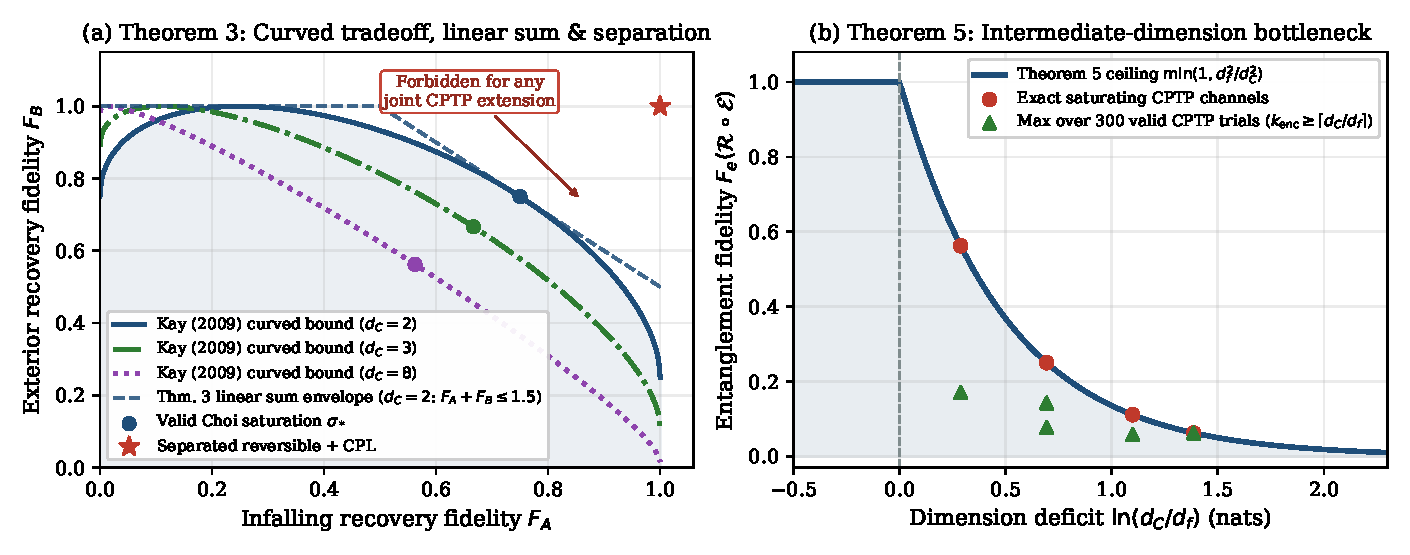
\includegraphics[width=\linewidth]{figures/fig2_joint_vs_separated.pdf}
  \caption{(a)~Theorem~\ref{thm:cpl}: exact curved upper boundaries \eqref{eq:kay-curved} plotted for $d_C=2,3,8$ (cf.\ \cite{Kay2009,Nechita2021}), together with the reverse-triangle lower boundary and constructively attainable shaded joint region shown for $d_C=2$ only (meeting at $F_B=1/4$ when $F_A=1$), linear sum outer envelope $F_A+F_B\le 1+1/d_C$ for $d_C=2$ (dashed tangent), valid CPTP Choi saturation points $\sigma_*$ \eqref{eq:choi-witness}, and the separate-condition reversible point $(1,1)$ (red star). (b)~Theorem~\ref{thm:bottleneck} (maximally mixed case of \cite{FarberGour2026}): sharp unassisted bottleneck ceiling $\min(1, d_f^2/d_C^2)$ with exact saturating CPTP channels (red circles), maxima over 300 random valid CPTP channels per $(d_C,d_f)$ pair ($k_{\mathrm{enc}} = \max(2,\lceil d_C/d_f\rceil)$, green triangles; TP residuals $\le 2.07\times 10^{-15}$), and the $(d_C=4, d_f=2)$ 1-bit classical-flag violation $F_e = 0.5 > 0.25$ (open purple diamond) illustrating the no-side-channel resource assumption.}
  \label{fig:joint-bottleneck}
\end{figure}

%==============================================================================
\section{Two-Window Compatibility Model, Companion Matrix Benchmark, and Numerical Audit}\label{sec:matrix}
%==============================================================================

To audit Theorems~\ref{thm:bps}--\ref{thm:bottleneck} and all structural counterexamples numerically, our companion script \code{scripts/\allowbreak verify\_\allowbreak ostqd.py} (fixed seed \code{20261126}; pinned environment in \code{scripts/\allowbreak require\-ments.txt}: Python~3.14.7, NumPy~2.4.2, SciPy~1.17.1, Matplotlib~3.10.8; 451~recorded scientific numeric fields in \code{docs/\allowbreak numerical\_\allowbreak verification.json}) performs three explicitly separated verifications:

\begin{enumerate}
  \item \textbf{Direct theorem, boundary-example, and counterexample checks (Theorems~\ref{thm:bps}--\ref{thm:bottleneck}):}
  We verify every identity and counterexample discussed in Sections~\ref{sec:framework}--\ref{sec:double-bottleneck}: the Definition~\ref{def:ostqd} $D_2\otimes M_2$ algebra non-closure counterexample (initial subalgebra diff $0.0$, time-$t$ split $\pm\sin(2t)$ exact), amplitude-damping BPS sufficiency vs.\ integrability ($[\cL,\ad_H]=0$ to $0.0$ while $\cL^\dagger(H)=-H$), degenerate-subspace non-Hermitian BPS purity increase ($2\Tr[\rho\cL(\rho)]=+0.25$ at $[L,H]=0$), maximally mixed drift cancellation ($\partial_s\mathrm{Var}_{\rho_{\mathrm{mm}}}(H_A)=0$ vs.\ $\langle\Gamma\rangle_{\rho_{\mathrm{mm}}}=4$ vs.\ eigenbasis average $4$), the nonzero-drift zero-covariance example ($H=\mathrm{diag}(0,1,2)$, $L=|2\rangle\langle 1|$, $\rho=\1_3/3$), the non-commuting PDE norm $2\sqrt{2}$, two-sided $[H_A,H_B]=0$ vs.\ exterior-local $\gamma_{\mathrm{loc}} = 8\omega^2 n_{\mathrm{FD}}(1-n_{\mathrm{FD}})$, one-sided reduced-state invariance ($\Tr_L$ and $\Tr_R$, error $0.0$), Gaussian phase-noise equivalence ($8.44\times 10^{-17}$), the $\gamma_{\mathrm{loc}}=2$ fixed-ground-state counterexample, the $s<0$ negative even-block subdeterminant ($-0.1216$ at $s=-0.5$), proportional-redshift visibility decay $\langle\sigma_x\rangle_{s=2}=e^{-1}$, the non-unital GKSL check, valid CPTP Choi saturation across the entire shaded achievable region---audited deterministically across $d\in\{2,3,5,8\}$ at 170 $(d,x)$ pairs (510 upper, lower, and interior Choi states; marginal error $\le 3.56\times 10^{-16}$, fidelity error $\le 1.00\times 10^{-15}$) alongside zero violations over 500 random pure states per dimension ($d=2,3,4,5$; 2,000 total)---the causal projective shared-record readout ($P(x\neq y)=0$, marginal error $1.67\times 10^{-16}$), the finite-$s$ weak $Z$-record measurement contrast at $\Gamma s = 1$ (non-selective match to phase damping $0.0$, universal disagreement probability $0.183940$, off-diagonal $|+\rangle\langle +|$ entry $0.303265$ vs.\ $0.0$ for projective pinching), the 1,500-trial random CPTP bottleneck test ($k_{\mathrm{enc}} = \max(2, \lceil d_C/d_f\rceil)$, TP residuals $\le 2.07\times 10^{-15}$), $d_f>d_C$ isometric saturation ($F_e=1.0$), and the $(d_C=4,d_f=2)$ 1-bit classical-flag violation ($F_e=0.5 > 0.25$).
  For Petz recovery evaluations below, given the normalized Choi state $J = d_C^{-1}\sum_\alpha |E_\alpha\rangle\!\rangle\langle\!\langle E_\alpha|$ and output marginal $\sigma = \mathcal{N}(\1_{d_C}/d_C)$, $\sigma^{-1/4}$ denotes the Moore--Penrose inverse power restricted to $\mathrm{supp}(\sigma)$; we cross-check $F_e(\cR_{\mathrm{Petz}}\circ\mathcal{N}) = \frac{1}{d_C}\Tr\bigl[((I\otimes\sigma^{-1/4})J(I\otimes\sigma^{-1/4}))^2\bigr]$ against explicit recovery Kraus operators $R_\alpha = d_C^{-1/2}E_\alpha^\dagger\sigma^{-1/2}$ (on $\mathrm{supp}(\sigma)$) over 100 random channels (max discrepancy $3.22\times 10^{-15}$), emphasizing that each Petz curve represents an explicit decoder's achieved fidelity rather than a channel-independent upper bound.

  \item \textbf{Piecewise time-dependent two-window $N=8$-qubit compatibility model (connecting Theorem~\ref{thm:double}(e)--(f) with Petz decoding):}
  To exhibit non-stationary intra-window $t$-encoding alongside exact Window-1 $s$-invariance and inter-window dephasing inside a \emph{single} Hilbert space, we construct $\cH_{\mathrm{tot}} = \cH_{\mathrm{win},1} \oplus \cH_{\mathrm{win},2} \cong \bbC^{256} \oplus \bbC^4$ with reference window Hamiltonian $H_{\mathrm{tot}} = H_{\mathrm{win},1} \oplus H_{\mathrm{win},2}$, where $H_{\mathrm{win},1}$ is a non-scalar GUE matrix linearly rescaled into $[E_1-\Delta, E_1+\Delta] = [0.8, 1.2]$ ($E_1=1.0, \Delta=0.2$) and $H_{\mathrm{win},2}$ lies in $[2.8, 3.2]$ ($E_2=3.0$). In dimensionless normalized units (writing $K_B = \sqrt{\kappa}(E_1\Pi_1 + E_2\Pi_2)$ with $\kappa=1$ so $s\kappa(E_1-E_2)^2$ is dimensionless in physical units), the coarse-grained actualization jump $K_B = E_1\Pi_1 + E_2\Pi_2$ obeys $\normF{[K_B, H_{\mathrm{tot}}]} = 0.0$.
  Inside Window~1 ($N=8$ qubits), we prepare a young black hole carrying one logical qubit maximally entangled with an external reference $R_{\mathrm{ref}}$ ($d_C=2$): $|\Psi(0)\rangle = \frac{1}{\sqrt{2}}(|0\rangle_{\mathrm{ref}}|0\rangle_{\mathrm{BH}} + |1\rangle_{\mathrm{ref}}|1\rangle_{\mathrm{BH}})$, where basis index $1$ places the initial logical qubit on the least-significant qubit (which is the first qubit transferred to the radiation register at step $k=1$). The reduced 256D Window-1 state $\rho_{\mathrm{win},1}(k) := \Tr_{R_{\mathrm{ref}}}|\Psi(k)\rangle\langle\Psi(k)|$ obeys $\normF{[H_{\mathrm{win},1}, \rho_{\mathrm{win},1}(0)]} = 0.0995 > 0$. Evolution across steps $k=1,\dots,8$ uses the piecewise time-dependent Hamiltonian
  \[
    H_{\mathrm{dyn}}(t) =
    \begin{cases}
      H_{\mathrm{win},1} \oplus H_{\mathrm{win},2}, & k = 1\;(\Delta t = 25),\\
      \bigl(H_{\mathrm{loc},k} \otimes \1_{\mathrm{rad},k-1}\bigr) \oplus H_{\mathrm{win},2}, & k = 2,\dots,8\;(\Delta t = 2),
    \end{cases}
  \]
  where ``local'' in $H_{\mathrm{loc},k}$ means specifically a dense GUE matrix acting on all $8-k+1$ remaining black-hole qubits while acting trivially on the $k-1$ already-emitted radiation qubits (not spatial $k$-locality on a lattice). Because $[K_B, H_{\mathrm{dyn}}(t)] = 0$ on every interval ($0.0$), the time-ordered unitary channel $\cU(t,t_0)$ commutes identically with $\Phi_B(s) = e^{s\cL_B}$, and $\normF{\cL_B(\rho_{\mathrm{win},1}(k))} = 0.0$ across all $k=0,\dots,8$.
  \emph{What drives Figure~\ref{fig:matrix} vs.\ inter-window $s$-decay and $d_C=4$ bottleneck contrasts:} Because $K_B = E_1\Pi_1$ acts as a scalar on Window~1, $\id_{R_{\mathrm{ref}}}\otimes\Phi_B(s)$ acts as the identity on all Window-1 states; setting $K_B=0$ yields analytically identical radiation entropy and Petz recovery curves in Figure~\ref{fig:matrix}, which are driven entirely by the piecewise GUE unitaries and radiation splits. Figure~\ref{fig:matrix} therefore serves specifically as a \emph{compatibility demonstration} of $t$-encoding/recovery with Window-1 $s$-invariance (and instantaneous $[K_B,H_{\mathrm{dyn}}(t)]=0$ ensures $s$-invariance while remaining distinct from $t$-direction energy conservation, as seen from $\Delta\langle H_{\mathrm{win},1}\rangle = +0.00236$ at $k=2$). To test the complementary effects directly, our script executes two explicit contrasts: (i)~encoding a logical qubit \emph{across} Window~1 and Window~2 ($|0_L\rangle\in\cH_{\mathrm{win},1}, |1_L\rangle\in\cH_{\mathrm{win},2}$) causes $s$-dephasing to degrade entanglement fidelity exactly as $F_e(s) = \frac{1}{2}(1+e^{-(E_1-E_2)^2 s/2})$ ($1.0 \to 0.5677$ at $s=1$, $0.5012$ at $s=3$; match $<10^{-15}$), while intra-window encoding remains invariant; and (ii)~encoding $d_C=4$ (two logical qubits) into the same $N=8$-qubit Window-1 model exercises Theorem~\ref{thm:bottleneck}'s nontrivial intermediate ceiling \emph{prior} to complete evaporation: at $k=7$ ($d_{\mathrm{rem}}=2 < d_C=4$), the ceiling drops below $1$ to $0.25$ with observed $F_{\mathrm{rem}}(7) = 0.0660 \le 0.25$, followed by exact saturation at complete erasure $F_{\mathrm{rem}}(8) = 0.0625 = 1/16$ at $k=8$ (note that the $d_C=4$ check shares the $k=1$ unitary while using independent GUE draws for $k\ge 2$, which suffices to audit the channel-independent ceiling; attributing step-by-step curve differences solely to $d_C$ would require identical GUE draws).

  \item \textbf{Independent companion $SU(2)$ Yang--Mills 2-matrix fixed-cutoff Galerkin benchmark:}
  Decoupled from the $N=8$-qubit model above, we compute the \emph{exact Galerkin eigenvalues at fixed Fock truncation $N_{\mathrm{cut}} = 3$} in the $SO(3)$ gauge-singlet sector of the bosonic two-matrix $SU(2)$ Yang--Mills Hamiltonian \cite{BFSS1997,IKKT1997}
  \[
    H_{\mathrm{YM}} = \tfrac{1}{2}\sum_{a=1}^3\bigl(P_{1,a}^2 + P_{2,a}^2\bigr) + \tfrac{1}{2}g_{\mathrm{YM}}^2\sum_{a=1}^3 \bigl((X_1 \times X_2)_a\bigr)^2 + \tfrac{1}{2}m^2\sum_{a=1}^3\bigl(X_{1,a}^2 + X_{2,a}^2\bigr)
  \]
  ($g_{\mathrm{YM}}=0.8, m=0.35$). Because each coordinate/momentum factor shifts total oscillator quanta by at most $\pm 1$, any four-factor path starting and ending at quanta $\le N_{\mathrm{cut}}$ cannot exceed intermediate quanta $N_{\mathrm{cut}}+2$; thus building the quartic polynomial at $N_{\mathrm{int}}=5$ (verified identical to $N_{\mathrm{int}}=6$ to $0.0$) certifies exact construction of the projected $N_{\mathrm{cut}}=3$ matrix (84D Fock space, 4D exact $SO(3)$ singlet kernel of $\mathbf{J}_{\mathrm{exact}}^2$), \emph{not} convergence to the continuum limit. The exact $N_{\mathrm{cut}}=3$ Galerkin singlet eigenvalues are $\{2.1436, 3.6063, 3.6063, 4.2664\}$ (compared with naive pre-truncated operator-product energies $\{2.1316, 2.8063, 2.8063, 3.4784\}$; singlet matrix Frobenius diff $1.3856$, eigenvalue $L^2$ diff $1.3788$). Increasing the target projection to $N_{\mathrm{cut}}=4$ (using $N_{\mathrm{int}}=6$, singlet dimension $10$) shifts the lowest four Galerkin eigenvalues to $\{2.0653, 3.5729, 3.5729, 3.8452\}$, confirming that continuum convergence requires substantially larger $N_{\mathrm{cut}}$ and that this benchmark serves solely as a finite-cutoff matrix-projection check rather than evidence of quantum chaos or the large-$N$ black-hole regime.
\end{enumerate}

\begin{figure}[!tbp]
  \centering
  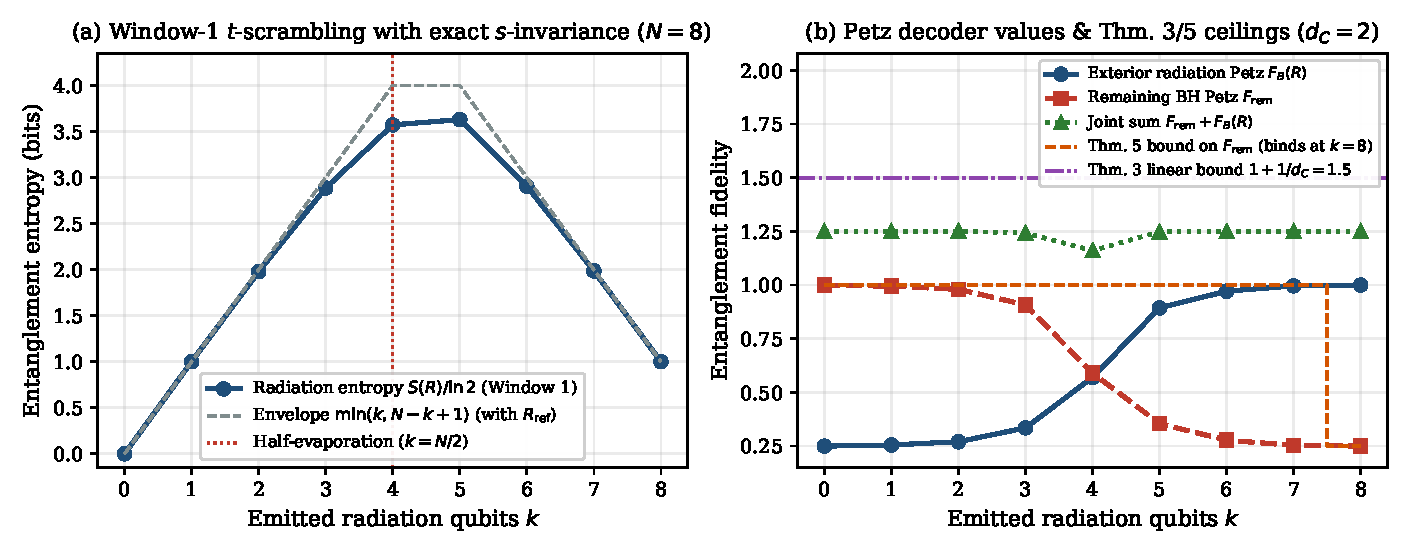
\includegraphics[width=0.95\linewidth]{figures/fig3_matrix_evaporation.pdf}
  \caption{Compatibility demonstration of piecewise time-dependent Window~1 $t$-scrambling ($N=8$ qubits; $d_C=2$, initial logical qubit at index~1 emitted first, joint BH--$R_{\mathrm{ref}}$ state pure) with exact coarse-grained $s$-invariance ($\normF{\cL_B(\rho_{\mathrm{win},1}(k))}=0$; setting $K_B=0$ yields analytically identical curves inside Window~1, whereas inter-window logical encoding decays as $\frac{1}{2}(1+e^{-\Delta E^2 s/2})$). (a)~Radiation entropy $S(R)/\ln 2$ bounded by $\min(k, 9-k)$ ($3.5720$~bits at $k=4$, $3.6294$~bits at $k=5$, ending at $1.0$~bit due to $R_{\mathrm{ref}}$). (b)~Petz transpose decoder values $F_B(R)$ ($0.2500\to 1.0000$) and $F_{\mathrm{rem}}$ ($1.0000\to 0.2500$); $\max_k F_{\mathrm{sum}}(k) \approx 1.250543 < 1.5$ (Theorem~\ref{thm:cpl}), while Theorem~\ref{thm:bottleneck}'s ceiling on $F_{\mathrm{rem}}$ (orange dashed step) equals $1.0$ for $k\le 7$ and saturates at $0.25$ at $k=8$ (for $d_C=4$, the ceiling already becomes nontrivial ($<1$) at $k=7$ with $F_{\mathrm{rem}}(7)=0.0660 < 0.25$ and saturates at $1/16$ at $k=8$; see text).}
  \label{fig:matrix}
\end{figure}

As shown in Figure~\ref{fig:matrix}, because the 1-qubit external reference $R_{\mathrm{ref}}$ purifies the initial 8-qubit black hole state (so the joint BH+$R_{\mathrm{ref}}$ system is initially pure with $N+1=9$ qubits), the radiation entropy $S(R)/\ln 2$ tracks the symmetric envelope $\min(k, 9-k)$ (attaining $3.5720$~bits at $k=4$ and $3.6294$~bits at $k=5$, and ending at $1.0$~bit at $k=8$ rather than $0$ bits). Note that this setup illustrates information release from an initially young black hole across half-evaporation, distinct from Hayden and Preskill's \cite{HaydenPreskill2007} rapid-mirror protocol for a diary thrown into an already old maximally entangled black hole. Likewise, for $d_C = 2$ and $d_f = 2^{8-k}$, Theorem~\ref{thm:bottleneck}'s bottleneck ceiling $\min(1, d_f^2/d_C^2)$ equals $1$ throughout $k=0,\dots,7$ and saturates at $1/4$ at complete evaporation $k=8$, whereas the $d_C=4$ contrast above exercises a nontrivial intermediate ceiling $1/4$ already at $k=7$ (with $F_{\mathrm{rem}}(7)=0.0660 < 0.25$, saturating at $1/16$ at $k=8$). Table~\ref{tab:numerics} summarizes all numerical audit residuals.

\begin{table}[!tbp]
\centering\scriptsize
\caption{Summary of deterministic numerical checks (\code{scripts/verify\_\allowbreak ostqd.py}, seed \code{20261126}, 451 recorded numeric fields; pinned versions in \code{scripts/requirements.txt}).}
\label{tab:numerics}
\begin{tabular}{@{}>{\raggedright\arraybackslash}p{0.34\linewidth}>{\raggedright\arraybackslash}p{0.35\linewidth}r@{}}
\toprule
Verification item & Theoretical identity / value & Observed error / value \\
\midrule
Def.~\ref{def:ostqd} $D_2\otimes M_2$, amp.-damp.\ \& deg.\ non-Herm. & $\pm\sin(2t)$; $[\cL,\ad_H]=0$, $\cL^\dagger(H)=-H$; $2\Tr(\rho\cL\rho)=+0.25$ & Exact ($0.0$) / $+0.25$ \\
Thm.~\ref{thm:bps}(a,c,d--f): Carr\'e du champ, BPS \& eig-avg & $\Gamma_{\cL}=\sum [L_k,H]^\dagger[L_k,H]$; eig.\ avg.\ $2.27\times 10^{-13}$, indiv.\ $2.84\times 10^{-13}$ & $\le 2.85\times 10^{-13}$ \\
Drift cancellation ($\1_2/2$) \& nonzero-$D$ zero-cov ($\1_3/3$) & $\partial_s\mathrm{Var}_{\mathrm{mm}}=0$ vs.\ $4$; $\partial_s\mathrm{Var}_{3}=\langle\Gamma\rangle_3=1/3$ & Exact ($<10^{-14}$) \\
Non-commuting PDE ($H=\sigma_z$, $L=\sigma_x$, $|+\rangle\langle +|$) & $\normF{\cL([H,\rho])-[H,\cL(\rho)]}=2\sqrt{2}$ & $2.828427$ \\
Thm.~\ref{thm:horizon}(d,e): 2-lvl $\gamma$, 4D $[H_A,H_B]=0$, $\gamma_{\mathrm{loc}}$ & $[H_A,H_B]=0$, $\gamma_{\mathrm{loc}}=8\omega^2 n_{\mathrm{FD}}(1-n_{\mathrm{FD}})$ & $\le 4.44\times 10^{-16}$ \\
Thm.~\ref{thm:horizon}(f): 4D ODE, direct rate, $\Tr_L/\Tr_R$, phase & Eqs.~\eqref{eq:ferm-energy-s}--\eqref{eq:firewall-entropy}; direct rate $5.55\times 10^{-17}$; $\theta\sim\mathcal{N}(0,\Gamma s)$ & $\le 2.22\times 10^{-16}$ \\
Fixed-ground counterex.\ ($\gamma_{\mathrm{loc}}=2$) \& $s=-0.5$ det & $\cL(|00\rangle\langle 00|)=0$ (eig-avg $=0.5$); $\det_{\mathrm{even}}<0$ & $0.0$ / $-0.121635$ \\
Bosonic pair ($N_{\mathrm{cut}}=18$, $T_H/\omega \le 0.8$ vs.\ $2.5$) & Eq.~\eqref{eq:unified-heating} ($\sigma=+1$); exact $N(1-q)q^{N-1}/(1-q^N)$ & $7.58\times 10^{-9}$ / $6.61\times 10^{-3}$ \\
Proportional redshift ($H_B=2H_A$, $L=H_A$, $s=2$) & $\gamma=0$, yet $\langle\sigma_x\rangle_2 = e^{-1}$ & $0.367879$ (exact) \\
Thm.~\ref{thm:cpl}(a--e): Full-band 510-pt Choi, proj.\ \& weak & Marg.\ $\le 3.56\times 10^{-16}$; proj.\ $0$ vs.\ weak dis.\ $0.183940$ & Fid.\ $\le 1.00\times 10^{-15}$ \\
Thm.~\ref{thm:double}(a,b,e): Parisi--Wu, Pyth., block decay & Eq.~\eqref{eq:block-eigen} \& $S_L(\cP\rho)=S_L(\rho)+\normF{\rho-\cP\rho}^2$ & $\le 1.11\times 10^{-16}$ \\
Thm.~\ref{thm:bottleneck}: 1,500 CPTP, $d_f>d_C$ \& classical flag & $F_e\le\min(1,d_f^2/d_C^2)$ (TP $\le 2.07\times 10^{-15}$); flag $F_e$ & 0 viol. / $0.500000$ \\
Petz Choi vs.\ explicit Kraus (100 random trials) & $F_e(\cR_{\mathrm{Petz}}\circ\mathcal{N})$ cross-check on $\mathrm{supp}(\sigma)$ & $3.22\times 10^{-15}$ \\
2-window BH ($N=8$): $d_C=2$, $d_C=4$ \& inter-window $s$ & $\max F_{\mathrm{sum}}=1.2505$; $d_C=4$ $F_{\mathrm{rem}}(7)=0.0660$; $F_e(1)=0.5677$ & $\normF{\cL_B}=0.0$ (Win.~1) \\
Companion $SU(2)$ YM Galerkin ($N_{\mathrm{cut}}=3$ vs.\ $4$) & $N_{\mathrm{cut}}=3$: $\{2.144,3.606,3.606,4.266\}$; $N_{\mathrm{cut}}=4$: $2.065\dots 3.845$ & $N_{\mathrm{int}}=5$ vs.\ $6$: $0.0$ \\
\bottomrule
\end{tabular}
\end{table}

%==============================================================================
\section{Scope, Analog Tests, and Open Problems Toward Quantum Gravity}\label{sec:discussion}
%==============================================================================

Returning to the motivating Hawking-evaporation observer-discrepancy paradox, we summarize clearly the conceptual and mathematical contributions achieved by OSTQD alongside what remains open:
\begin{itemize}
  \item \textbf{Conceptual contribution:} Rather than treating the operational mismatch between an infalling observer's locally smooth interior evolution and an asymptotic observer's directly accessible Hawking-evaporation records merely as an inconsistency to eliminate, we use this observer-dependent divergence of futures as an organizing principle to construct an explicit observer-indexed $(t,s)$ algebraic framework separating reversible clock-time unitarity from irreversible non-selective auxiliary-time dissipation, while specifying explicitly when evolution closes on a fixed subalgebra ($[H_O,\cA_O]\subseteq\cA_O$) versus acting by global-state restriction.
  \item \textbf{What is rigorously proved (conditional finite-dimensional core):} Under the explicit hypotheses of Definition~\ref{def:ostqd} and Theorems~\ref{thm:bps}--\ref{thm:bottleneck}, (i)~for purely dissipative GKSL generators, BPS energy-moment conservation is equivalent to $[L_k,H]=0$ and is sufficient (not necessary) for $(t,s)$ integrability, while $\frac{1}{d}\Tr\Gamma_{\cL}(H,H)$ measures the exact eigenbasis-averaged initial variance rate; (ii)~in the 4D fermionic Hawking pair, although $[H_A,H_B]=0$ globally, restricting exterior jumps to $\cA_B = M_2(\bbC)_R\otimes\1_L$ forces local incompatibility $\gamma_{\mathrm{loc}} = 8\omega^2 n_{\mathrm{FD}}(1-n_{\mathrm{FD}}) > 0$ for $T_H>0$ and excites the \emph{two-sided} observable $H_A$ on $|0_A\rangle$ at rate \eqref{eq:unified-heating} while leaving both one-sided reduced states ($\Tr_L\rho_B(s)$ and $\Tr_R\rho_B(s)$) invariant (with a 4D counterexample showing $\gamma_{\mathrm{loc}}>0$ alone does not guarantee ground-state heating); (iii)~for $d_C\ge 2$, any global joint CPTP extension obeys both the curved upper/lower boundaries \eqref{eq:kay-curved} \cite{Kay2009,Nechita2021}---with the entire shaded band constructively attained by valid CPTP Choi states---and the linear outer envelope $F_A+F_B \le 1+1/d_C$, whereas separate-condition reversible channels with inverse decoders achieve $F_e=1$ each with marginal consistency on $\cA_{\mathrm{sh}}$ and single-trial agreement on a commuting classical-record factor via the ideal projective readout of Theorem~\ref{thm:cpl}(e) (matching the $s\to\infty$ record limit and contrasted explicitly with finite-$s$ weak measurement); (iv)~sector-separating commuting spectral Hermitian jumps drive $e^{s\cL} \to \cP$ exponentially and preserve nontrivial intra-window $t$-evolution inside a finite-width energy window $\Pi_{\mathrm{win}}$; and (v)~as the maximally mixed special case of Farber and Gour's unassisted single-shot compression theorem \cite{FarberGour2026}, intermediate Hilbert spaces of dimension $d_f$ without classical side channels or radiation access cap entanglement fidelity sharply at $\min(1, d_f^2/d_C^2)$ (exceeded to $1/2>1/4$ when a 1-bit classical flag is allowed).
  \item \textbf{Analog quantum-simulator tests vs.\ genuine quantum-gravity predictions:} The conditional channel identities \eqref{eq:unified-heating} and \eqref{eq:joint-bound}--\eqref{eq:kay-curved} can be tested in controllable two-mode squeezing platforms with engineered dephasing $\Gamma s$. However, because the single-mode channel $\Phi_B(s)$ is operationally indistinguishable from ordinary Gaussian phase noise or unitary environmental coupling (Remark~\ref{rem:horizon-scope}), such experiments test the channel algebra rather than gravitational actualization. Predicting a genuinely gravitational signature requires specifying normalized wavepackets, detector-field coupling, a microscopic derivation of $\Gamma_{\mathrm{eff}}(\tau) = \Gamma_O\,ds/d\tau$, and an observable distinguishing the model from standard unitary environmental decoherence.
  \item \textbf{Open nonperturbative problems:} Lifting finite-dimensional matrix semigroups to infinite-dimensional Type~$\mathrm{II}_1/\mathrm{II}_\infty$ crossed-product von Neumann algebras \cite{CLPW2023,DeVuyst2025} (which requires specifying the semifinite trace, unbounded generator domain, and continuity topology); computing renormalized continuum horizon stress-energy tensors, Hadamard regularity, and wavepacket detector response; formulating general observer-separated selective instruments $\{\cI_{O,x}\}$ and causal record-merging rules beyond commuting classical-record factors; deriving $\Gamma_O$ and $s(\tau)$ microscopically from large-$N$ BFSS/IKKT matrix dynamics \cite{BFSS1997,IKKT1997,Choudhury2024} without external clock oracles; and clarifying how a smooth 4D Lorentzian spacetime manifold emerges from observer-indexed algebraic networks. These remain open research problems rather than solved claims of the present work.
\end{itemize}

%==============================================================================
\section{Lean~4 Formal Verification and Honest Scope Audit}\label{sec:lean}
%==============================================================================

The finite-dimensional algebraic core of Theorems~\ref{thm:bps}--\ref{thm:bottleneck} and the accompanying structural counterexamples are formalized over complex matrix algebras \code{Matrix (Fin d) (Fin d) $\bbC$} and \code{Matrix (TriIdx d) (TriIdx d) $\bbC$} in \textbf{Lean~4.36.0} with \textbf{Mathlib4} (\code{rev = v4.36.0}), comprising \textbf{50~audited public theorem declarations} across six modules (\code{Basic}, \code{Theorem1\_\allowbreak BPS}--\code{Theorem5\_\allowbreak Bottleneck}, alongside internal helper lemmas). A complete reproducible kernel build log (\code{lake build OSTQD}, \code{lake env lean OSTQD/\allowbreak AxiomCheck.lean}, and static forbidden-token audit via \code{lean4/verify\_lean.sh}) is bundled in \code{lean4/\allowbreak VERIFICATION\_\allowbreak LOG.txt}: all 50 audited declarations pass with zero errors, zero tactic-linter warnings (distinct from Lean~4.36.0's benign \code{module}-system import notice), zero \code{sorry}/\allowbreak\code{admit}/\allowbreak\code{axiom}/\allowbreak\code{constant}/\allowbreak\code{unsafe}/\allowbreak\code{sorryAx}, and depend exclusively on Lean's three standard axioms (\code{propext}, \code{Classical.choice}, \code{Quot.sound}).

Crucially, to avoid overstating what machine verification guarantees, Table~\ref{tab:lean} explicitly separates the \emph{Lean-verified algebraic core} from the \emph{standard analytic/hand-proved steps and physical hypotheses} that lie outside the Lean formalization.

\begin{table}[!tb]
\centering\scriptsize
\caption{Exact correspondence between manuscript claims, Lean~4.36.0 formalized algebraic core (50 audited public declarations; full kernel log in \code{lean4/\allowbreak VERIFICATION\_\allowbreak LOG.txt}), and analytic/physical steps outside Lean.}
\label{tab:lean}
\begin{tabular}{@{}>{\raggedright\arraybackslash}p{0.13\linewidth}>{\raggedright\arraybackslash}p{0.46\linewidth}>{\raggedright\arraybackslash}p{0.34\linewidth}@{}}
\toprule
Paper result & Lean~4.36.0 formalized algebraic core (module \& declarations) & Analytic / physical steps outside Lean \\
\midrule
GKSL basics (\S\ref{sec:framework}) & \code{Basic.lean} (2): \code{trace\_\allowbreak gksl\_\allowbreak eq\_\allowbreak zero}, \code{gksl\_\allowbreak dual\_\allowbreak adj}: generator trace preservation and Schr\"odinger--Heisenberg duality on $M_d(\bbC)$. & Matrix exponential $\Phi_O(s)=e^{s\cL_O}$, CPTP semigroup generation, general selective instruments $\{\cI_{O,x}\}$. \\
Theorem~\ref{thm:bps} & \code{Theorem1\_\allowbreak BPS.lean} (10): \code{carre\_\allowbreak du\_\allowbreak champ\_\allowbreak eq\_\allowbreak sum\_\allowbreak comm\_\allowbreak sq}, \code{carre\_\allowbreak du\_\allowbreak champ\_\allowbreak trace\_\allowbreak nonneg}, \code{bps\_\allowbreak immunity\_\allowbreak iff\_\allowbreak comm}, \code{two\_\allowbreak time\_\allowbreak commutation}, \code{variance\_\allowbreak deriv\_\allowbreak exact\_\allowbreak decomp}, \code{eigenstate\_\allowbreak variance\_\allowbreak deriv\_\allowbreak eq\_\allowbreak carre\_\allowbreak du\_\allowbreak champ}, \code{eigenbasis\_\allowbreak sum\_\allowbreak variance\_\allowbreak deriv\_\allowbreak eq\_\allowbreak trace\_\allowbreak carre\_\allowbreak du\_\allowbreak champ}, \code{algebra\_\allowbreak nonclosure\_\allowbreak counterexample}, \code{bps\_\allowbreak sufficient\_\allowbreak not\_\allowbreak necessary\_\allowbreak for\_\allowbreak commutation}, \code{nonhermitian\_\allowbreak bps\_\allowbreak degenerate\_\allowbreak purity\_\allowbreak increase}. & Analytic passage from $[\cL,\ad_H]=0$ to $\cU(t)\circ\Phi(s)=\Phi(s)\circ\cU(t)$; chain-rule link (\code{HasDerivAt}) connecting algebraic \code{varianceDeriv} to $\partial_s \mathrm{Var}_{\rho(s)}(H)|_{s=0}$ along $e^{s\cL}$. \\
Theorem~\ref{thm:horizon} & \code{Theorem2\_\allowbreak Horizon.lean} (16): \code{universal\_\allowbreak actualization\_\allowbreak nogo}, \code{local\_\allowbreak actualization\_\allowbreak nogo}, \code{quantitative\_\allowbreak horizon\_\allowbreak heating\_\allowbreak bound}, \code{local\_\allowbreak dissipation\_\allowbreak bound}, \code{static\_\allowbreak redshift\_\allowbreak zero\_\allowbreak conflict}, \code{two\_\allowbreak level\_\allowbreak bogoliubov\_\allowbreak incompatibility}, \code{fermionic\_\allowbreak hawking\_\allowbreak HA\_\allowbreak comm\_\allowbreak HB}, \code{fermionic\_\allowbreak hawking\_\allowbreak local\_\allowbreak incompatibility}, \code{fermionic\_\allowbreak hawking\_\allowbreak local\_\allowbreak nogo}, \code{fermionic\_\allowbreak hawking\_\allowbreak HB\_\allowbreak bps\_\allowbreak immune}, \code{fermionic\_\allowbreak hawking\_\allowbreak ode} (\code{HasDerivAt}), \code{fermionic\_\allowbreak hawking\_\allowbreak energy\_\allowbreak at\_\allowbreak s}, \code{fermionic\_\allowbreak hawking\_\allowbreak firewall\_\allowbreak entropy\_\allowbreak identity}, \code{positive\_\allowbreak gamma\_\allowbreak loc\_\allowbreak fixed\_\allowbreak ground\_\allowbreak state\_\allowbreak counterexample}, \code{fermionic\_\allowbreak hawking\_\allowbreak reduced\_\allowbreak states\_\allowbreak invariant}, \code{fermionic\_\allowbreak hawking\_\allowbreak neg\_\allowbreak s\_\allowbreak not\_\allowbreak psd}. & Compactness minimization of $\gamma_{\mathrm{loc}}$; $s\to\infty$ limit ($\Gamma>0$); bosonic infinite-dimensional Fock series \eqref{eq:unified-heating}; physical justification of $\cA_B$, wavepackets, and continuum firewalls. \\
Theorem~\ref{thm:cpl} & \code{Theorem3\_\allowbreak CrossPerspective.lean} (10): \code{projA\_\allowbreak projB\_\allowbreak projA}, \code{joint\_\allowbreak extension\_\allowbreak fidelity\_\allowbreak bound} (pure), \code{joint\_\allowbreak extension\_\allowbreak fidelity\_\allowbreak bound\_\allowbreak mixed} (convex mixtures), \code{joint\_\allowbreak extension\_\allowbreak no\_\allowbreak simultaneous\_\allowbreak faithful}, \code{joint\_\allowbreak extension\_\allowbreak bound\_\allowbreak sharp} ($\sigma_*$), \code{observer\_\allowbreak separated\_\allowbreak cpl\_\allowbreak consistency}, \code{asymmetric\_\allowbreak kay\_\allowbreak choi\_\allowbreak saturation} ($\sigma^+(x)$), \code{shared\_\allowbreak causal\_\allowbreak record\_\allowbreak instrument\_\allowbreak agreement}, \code{achievable\_\allowbreak joint\_\allowbreak region\_\allowbreak choi\_\allowbreak complete} (full shaded band), \code{weak\_\allowbreak record\_\allowbreak measurement\_\allowbreak vs\_\allowbreak projective\_\allowbreak readout}. & Curved upper/lower boundary inequalities \eqref{eq:kay-curved} (hand-proved \& numerically verified \cite{Kay2009,Nechita2021}); Choi-channel operational correspondence; general black-hole record-merging rules. \\
Theorem~\ref{thm:double} & \code{Theorem4\_\allowbreak DoubleUncertainty.lean} (6): \code{parisi\_\allowbreak wu\_\allowbreak purity\_\allowbreak monotonicity}, \code{double\_\allowbreak uncertainty\_\allowbreak pythagorean}, \code{weak\_\allowbreak gravity\_\allowbreak invisibility}, \code{microcanonical\_\allowbreak code\_\allowbreak invariance}, \code{commuting\_\allowbreak jumps\_\allowbreak block\_\allowbreak eigenvalue} (Eq.~\eqref{eq:block-eigen}), \code{microcanonical\_\allowbreak window\_\allowbreak scrambling\_\allowbreak compatible} (Eq.~\eqref{eq:window-compat}). & Analytic limit $e^{s\cL}\to\cP$ (or $E_{\cF}$ for non-commuting jumps); von Neumann version $S(\cP\rho)=S(\rho)+D(\rho\|\cP\rho)$; scrambling correlation metrics. \\
Theorem~\ref{thm:bottleneck} & \code{Theorem5\_\allowbreak Bottleneck.lean} (6): \code{bottleneck\_\allowbreak entanglement\_\allowbreak fidelity\_\allowbreak bound}, \code{entanglement\_\allowbreak fidelity\_\allowbreak le\_\allowbreak one}, \code{bottleneck\_\allowbreak entanglement\_\allowbreak fidelity\_\allowbreak min\_\allowbreak bound}, \code{bottleneck\_\allowbreak bound\_\allowbreak sharp} ($0<d_f\le d_C$), \code{bottleneck\_\allowbreak bound\_\allowbreak sharp\_\allowbreak large\_\allowbreak df} ($0<d_C\le d_f$), \code{classical\_\allowbreak flag\_\allowbreak beats\_\allowbreak unassisted\_\allowbreak bottleneck}. & Choi-state equivalence of Kraus $F_e$; general mixed-state Ky Fan theorem \cite{FarberGour2026}; physical identification $\ln d_f \leftrightarrow S_{\mathrm{BH}}$ and distinction from BH mergers \cite{Hawking1971}. \\
\bottomrule
\end{tabular}
\end{table}

%==============================================================================
\section*{Author Contributions, AI Disclosure, and Reproducibility Provenance}\label{sec:ai-disclosure}
%==============================================================================
\addcontentsline{toc}{section}{Author Contributions, AI Disclosure, and Reproducibility Provenance}

Following transparent AI task disclosure practices in theoretical high-energy and matrix-model research \cite{Michel2026}, we explicitly separate human and AI contributions and document the verification provenance:
\begin{itemize}
  \item \textbf{Human author (Yohtaro Soga):} Conceived the core physical motivation and research direction---taking the observer-dependent divergence of accessible futures of an infalling body under Hawking evaporation as a clue for quantum gravity, proposing the separation of reversible unitary evolution ($t$) from observer-relative irreversible dissipation via a Parisi--Wu-like directed auxiliary parameter ($s$), specifying the distinction between Layer~1 open-system mixedness and Layer~2 auxiliary-time dissipation, setting strict mathematical and formal-verification standards, and directing the project.
  \item \textbf{AI research assistant (Google Antigravity / Gemini):} Assisted with the 2022--2026 literature survey and positioning, formulated and proved Theorems~\ref{thm:bps}--\ref{thm:bottleneck} and the accompanying counterexamples in their finite-dimensional algebraic form, wrote and executed the Python numerical verification and plotting scripts, authored and kernel-verified all Lean~4.36.0 / Mathlib4 formalization files, verified external bibliographic records, and assisted with LaTeX manuscript drafting and formatting.
\end{itemize}
\paragraph{Verification provenance.}
All 50 audited finite-dimensional algebraic declarations are machine-checked by the Lean~4.36.0 kernel against pinned Mathlib4 \code{v4.36.0} (\code{lean4/lake-manifest.json}; reproducible via \code{lean4/verify\_lean.sh}, archived in \code{lean4/VERIFICATION\_LOG.txt}). All 451 recorded numeric fields, Table~\ref{tab:numerics}, and Figures~\ref{fig:heating}--\ref{fig:matrix} are deterministically reproduced from \code{scripts/verify\_ostqd.py} (seed \code{20261126}, single-threaded BLAS/OpenMP) in the pinned environment \code{scripts/requirements.txt} (Python~3.14.7, NumPy~2.4.2, SciPy~1.17.1, Matplotlib~3.10.8); exact trust boundaries and independent cross-checks are documented in \code{VERIFICATION.md} and \code{PRIOR\_ART.md}.

\bibliographystyle{unsrt}
\bibliography{references}

\end{document}
